\chapter{Implementation, Evaluation, and Results}
\label{chap:implementation}

This chapter presents the implementation of CORAL, the experimental methodology, and the empirical results of both project iterations. We first describe the technology stack, REST API, BK-tree construction, registry, and front-end. We then report the Iteration~1 (FYP-1) baseline results that informed the redesign, and finally present the Iteration~2 (FYP-2) results: large-scale evaluation on Common Voice Urdu, ablation study on Conversational Urdu, ensemble-size sensitivity, and OOV-threshold sensitivity. The chapter closes with a residual-error analysis.

\section{Implementation}
\label{sec:implementation}

\subsection{System Topology}
\label{ssec:topology}

CORAL is delivered as a four-tier system:

\begin{itemize}
  \item \textbf{Inference tier (Kaggle GPU notebooks).} Heavy ASR back-ends (Whisper-Large-v3, SeamlessM4T-v2-Large, optionally Whisper-Medium and Wav2Vec2-Urdu) run on Kaggle GPUs. Each notebook starts a small FastAPI inference server, exposes it through an ngrok HTTPS tunnel, self-registers with the backend's model registry, and sends 60-second heartbeats.
  \item \textbf{Backend pipeline tier (FastAPI).} A single \texttt{main\_app.py} mounts two routers: \texttt{pipeline\_api.py} (the \texttt{/health}, \texttt{/align}, \texttt{/oov}, \texttt{/correct} endpoints) and \texttt{registery\_api.py} (the \texttt{/registry/*} endpoints). Stages~0--3 of the pipeline run server-side here.
  \item \textbf{Front-end tier (Next.js + React).} The user-facing application implements a four-pass workflow (mode selection, alignment, OOV sieve, correction). Stage~4 (LLM refinement) is invoked from this tier so that user-supplied LLM API keys (Gemini, OpenRouter) never leave the browser.
  \item \textbf{Data tier (HuggingFace Hub + DuckDB).} The BK-tree (\texttt{bk\_tree.joblib}) and the n-gram tables (five Parquet files) are downloaded from a private HuggingFace bucket on first startup, cached locally, and loaded into a DuckDB connection.
\end{itemize}

\begin{figure}[H]
    \centering
    \resizebox{0.95\textwidth}{!}{%
    \begin{tikzpicture}[every node/.style={font=\small\sffamily}]
      % four tiers as horizontal swimlanes
      % --- Tier headings ---
      \node[coral/title, anchor=west] at (-3.6, 4.4) {Inference tier};
      \node[coral/title, anchor=west] at (-3.6, 2.4) {Backend tier};
      \node[coral/title, anchor=west] at (-3.6, 0.2) {Frontend tier};
      \node[coral/title, anchor=west] at (-3.6,-1.7) {Data tier};
      % swimlane separators
      \draw[coralGrey!50, thick, dashed] (-3.7, 3.5)  -- (24.5, 3.5);
      \draw[coralGrey!50, thick, dashed] (-3.7, 1.4)  -- (24.5, 1.4);
      \draw[coralGrey!50, thick, dashed] (-3.7,-0.7)  -- (24.5,-0.7);
      % Inference tier
      \node[coral/data, minimum width=32mm] (k1) at (3, 4.4)  {Kaggle GPU\\\scriptsize Whisper-Large-v3};
      \node[coral/data, minimum width=32mm] (k2) at (8.0, 4.4) {Kaggle GPU\\\scriptsize Seamless-Large};
      \node[coral/data, minimum width=32mm] (k3) at (13.0, 4.4) {Kaggle GPU\\\scriptsize Whisper-Medium};
      \node[coral/data, minimum width=32mm] (k4) at (18.0, 4.4) {Kaggle GPU\\\scriptsize Wav2Vec2-Urdu};
      \node[coral/api, minimum width=22mm] (ngrok) at (22.0, 4.4) {ngrok\\HTTPS};
      % Backend tier
      \node[coral/api, minimum width=44mm] (registry) at (4.5, 2.4) {\textbf{Model registry}\\\scriptsize /register /ping /transcribe};
      \node[coral/stage, minimum width=42mm] (align)  at (10.5, 2.4) {/align};
      \node[coral/stage, minimum width=42mm] (oov)    at (15.4, 2.4) {/oov};
      \node[coral/stage, minimum width=42mm] (correct) at (20.3, 2.4) {/correct};
      \node[coral/sublabel] at (15.4, 1.85) {FastAPI (Stages 0--3)};
      % Frontend tier
      \node[coral/api, minimum width=32mm] (mode)  at (3, 0.2)  {ModeSelector};
      \node[coral/api, minimum width=32mm] (p0)    at (7.6, 0.2) {Pass0Speech};
      \node[coral/api, minimum width=32mm] (p1)    at (11.6, 0.2){Pass1Input};
      \node[coral/api, minimum width=32mm] (p2)    at (15.6, 0.2){Pass2Sieve};
      \node[coral/api, minimum width=32mm] (p3)    at (19.6, 0.2){Pass3Correction};
      \node[coral/llm, minimum width=22mm] (llm)   at (23.0, 0.2){LLM\\Stage 4};
      % Data tier
      \node[coral/data, minimum width=42mm] (hf)    at (4.0, -1.7) {HuggingFace Hub\\\scriptsize bucket};
      \node[coral/data, minimum width=46mm] (bk)    at (10.5, -1.7) {BK-tree.joblib\\\scriptsize $\sim$50 MB};
      \node[coral/data, minimum width=58mm] (duck)  at (17.5, -1.7) {DuckDB n-gram tables\\\scriptsize bigram + trigram (5 Parquets)};
      % connections (vertical, between tiers)
      \draw[coral/arrow] (k1.south) -- (k1.south |- ngrok.south) -- (ngrok.west);
      \draw[coral/arrow] (k2.south) -- (k2.south |- ngrok.south) -- (ngrok.west);
      \draw[coral/arrow] (k3.south) -- (k3.south |- ngrok.south) -- (ngrok.west);
      \draw[coral/arrow] (k4.south) -- (k4.south |- ngrok.south) -- (ngrok.west);
      \draw[coral/arrow] (ngrok.south) -- (ngrok.south |- registry.north) -- (registry.east);
      \draw[coral/arrow] (registry.south) -- (registry.south |- p0.north) -- (p0.north);
      \draw[coral/biarrow] (align.south)   -- (align.south   |- p1.north) -- (p1.north);
      \draw[coral/biarrow] (oov.south)     -- (oov.south     |- p2.north) -- (p2.north);
      \draw[coral/biarrow] (correct.south) -- (correct.south |- p3.north) -- (p3.north);
      \draw[coral/biarrow] (llm.north) ++(0,3.5) -- (llm.north);
      \draw[coral/dashed] (hf.north)   -- (hf.north   |- registry.south);
      \draw[coral/dashed] (bk.north)   -- (oov.south);
      \draw[coral/dashed] (duck.north) -- (duck.north |- correct.south);
      % colour legend
      \node[coral/note, anchor=north west, align=left, text width=24cm] at (-3.7, -3.2)
        {\textbf{Legend.}\quad
         \tikz[baseline]\node[coral/data, minimum width=12mm]{\strut};\ inference / data\quad
         \tikz[baseline]\node[coral/api, minimum width=12mm]{\strut};\ HTTP API\quad
         \tikz[baseline]\node[coral/stage, minimum width=12mm]{\strut};\ pipeline stage\quad
         \tikz[baseline]\node[coral/llm, minimum width=12mm]{\strut};\ LLM.\quad
         Arrows: \emph{single} = unidirectional, \emph{double} = bidirectional, \emph{dashed} = data-tier dependency.};
    \end{tikzpicture}}
    \caption[CORAL four-tier system architecture]{CORAL four-tier system architecture. The \emph{Inference tier} runs heavy ASR back-ends on Kaggle GPUs and exposes them through ngrok HTTPS tunnels. The \emph{Backend tier} (FastAPI) hosts the registry plus the three stage endpoints. The \emph{Frontend tier} (Next.js) implements the four-pass user workflow and the Stage 4 LLM call. The \emph{Data tier} bootstraps the BK-tree and DuckDB n-gram tables from the HuggingFace bucket on startup.}
    \label{fig:system-architecture}
\end{figure}

\clearpage

\begin{figure}[H]
    \centering
    \resizebox{0.92\textwidth}{!}{%
    \begin{tikzpicture}[every node/.style={font=\small\sffamily}]
      % central registry
      \node[coral/api, minimum width=42mm, minimum height=18mm] (reg) at (8, 0)
            {\textbf{Backend}\\(FastAPI)\\\scriptsize main\_app.py};
      % Kaggle nodes around it
      \node[coral/data, minimum width=32mm] (k1) at (0, 3)   {Kaggle GPU 1\\\scriptsize Whisper-Large-v3};
      \node[coral/data, minimum width=32mm] (k2) at (16, 3)  {Kaggle GPU 2\\\scriptsize Seamless-Large};
      \node[coral/data, minimum width=32mm] (k3) at (0,-3)   {Kaggle GPU 3\\\scriptsize Whisper-Medium};
      \node[coral/data, minimum width=32mm] (k4) at (16,-3)  {Kaggle GPU 4\\\scriptsize Wav2Vec2-Urdu};
      % ngrok tunnels
      \node[coral/api, minimum width=18mm] (ng1) at (4, 1.6)  {ngrok};
      \node[coral/api, minimum width=18mm] (ng2) at (12, 1.6) {ngrok};
      \node[coral/api, minimum width=18mm] (ng3) at (4,-1.6)  {ngrok};
      \node[coral/api, minimum width=18mm] (ng4) at (12,-1.6) {ngrok};
      % browser
      \node[coral/entity, minimum width=34mm] (browser) at (24, 0)
            {End user browser\\\scriptsize Next.js front-end};
      % HF bucket
      \node[coral/data, minimum width=34mm] (hf) at (8, -5.2) {HuggingFace Hub\\\scriptsize private bucket};
      % connections
      \draw[coral/arrow] (k1) -- node[above, font=\scriptsize] {/transcribe} (ng1);
      \draw[coral/arrow] (k2) -- node[above, font=\scriptsize] {/transcribe} (ng2);
      \draw[coral/arrow] (k3) -- node[below, font=\scriptsize] {/transcribe} (ng3);
      \draw[coral/arrow] (k4) -- node[below, font=\scriptsize] {/transcribe} (ng4);
      \draw[coral/biarrow] (ng1.south) -- (reg.north west);
      \draw[coral/biarrow] (ng2.south) -- (reg.north east);
      \draw[coral/biarrow] (ng3.north) -- (reg.south west);
      \draw[coral/biarrow] (ng4.north) -- (reg.south east);
      \draw[coral/biarrow] (reg) -- node[above, font=\scriptsize] {REST API} (browser);
      \draw[coral/dashed]  (hf) -- node[right, font=\scriptsize] {bootstrap (once)} (reg);
      % heartbeat / fan-out callouts
      \node[coral/note, anchor=west, align=left] at (-2.5, 5)
            {\textbf{Self-registration}: Kaggle notebook POSTs\\
             \texttt{/registry/register} on startup with\\
             session\_id; pings every 60~s.};
      \node[coral/note, anchor=west, align=left] at (17, 5)
            {\textbf{Eviction}: registry sweep every 20~s\\
             removes models silent $>$300~s.};
      \node[coral/note, anchor=west, align=left] at (-2.5,-5.6)
            {\textbf{Fan-out}: \texttt{POST /registry/transcribe}\\
             dispatches audio to all live whitelisted\\
             models in parallel via \texttt{httpx.AsyncClient}\\
             with 60~s per-model timeout.};
      \node[coral/note, anchor=west, align=left] at (17,-5.6)
            {\textbf{Auth}: registration / ping require\\
             \texttt{X-Registry-Token}; transcribe requires\\
             \texttt{X-API-Token}.};
    \end{tikzpicture}}
    \caption[CORAL deployment topology]{CORAL deployment topology. Each ASR model runs on its own Kaggle GPU notebook with a private ngrok HTTPS tunnel; the backend registry is the rendezvous point. The browser talks only to the backend and (for Stage 4) directly to the LLM provider. The HuggingFace Hub bucket is read-only and consulted only at backend startup.}
    \label{fig:deployment-topology}
\end{figure}

\clearpage

\subsection{Technology Stack}
\label{ssec:tech-stack}

\begin{itemize}
  \item \textbf{Language and runtime:} Python 3.10+ for the backend; TypeScript / Node.js 20+ for the front-end.
  \item \textbf{Backend libraries:} \texttt{FastAPI 0.109}, \texttt{uvicorn 0.23}, \texttt{rapidfuzz 3.6} for Levenshtein distance, \texttt{joblib 1.3} for BK-tree serialisation, \texttt{duckdb 0.10} + \texttt{pyarrow 14} for n-gram queries, \texttt{huggingface\_hub 0.20} for data download, \texttt{httpx 0.26} for asynchronous fan-out, \texttt{pydantic 1.10} for request/response models, \texttt{python-dotenv 1.0} for configuration.
  \item \textbf{Front-end libraries:} \texttt{Next.js 14}, React, TailwindCSS, Axios. Stage~4 invocations talk directly to Google Generative Language API (Gemini) or OpenRouter chat-completions.
  \item \textbf{Inference libraries (Kaggle):} \texttt{transformers}, \texttt{torch}, \texttt{librosa}, \texttt{ngrok}.
  \item \textbf{Evaluation:} \texttt{jiwer} for WER/CER on the deployed pipeline; a custom evaluation harness for Iteration~1 ECE.
  \item \textbf{Visualisation:} \texttt{matplotlib} and \texttt{seaborn} for the figures in Section~\ref{sec:results-readspeech}.
\end{itemize}

\begin{figure}[H]
    \centering
    \resizebox{0.95\textwidth}{!}{%
    \begin{tikzpicture}[every node/.style={font=\small\sffamily}]
      % UML-style component diagram for the backend pipeline package
      % Outer "Backend" box
      \draw[coralBlue!50, very thick, rounded corners] (-0.5, -0.5) rectangle (24, 8.4);
      \node[coral/title, anchor=south west] at (-0.4, 8.45) {Backend (FastAPI)};
      % main_app
      \node[coral/api, minimum width=42mm] (main) at (3, 7.4) {\texttt{main\_app.py}\\\scriptsize FastAPI lifespan};
      % pipeline package
      \draw[coralOrange!50, thick, dashed, rounded corners] (0.2, 1.2) rectangle (12.5, 6.0);
      \node[coral/title, anchor=south west, text=coralOrange!60!black] at (0.3, 6.05) {pipeline/};
      \node[coral/stage, minimum width=44mm] (papi)  at (3.4, 5.2) {\texttt{pipeline\_api.py}};
      \node[coral/stage, minimum width=44mm] (pfun)  at (9.5, 5.2) {\texttt{coral\_pipeline\_functions.py}};
      \node[coral/stage, minimum width=44mm] (putil) at (3.4, 3.8) {\texttt{coral\_utility\_functions.py}};
      \node[coral/stage, minimum width=44mm] (pbk)   at (9.5, 3.8) {\texttt{bktree.py}};
      \node[coral/stage, minimum width=44mm] (pdl)   at (6.4, 2.2) {\texttt{coral\_data\_downloader.py}};
      % registry package
      \draw[coralViolet!50, thick, dashed, rounded corners] (13.5, 3.0) rectangle (23.7, 6.0);
      \node[coral/title, anchor=south west, text=coralViolet!60!black] at (13.6, 6.05) {model\_registery/};
      \node[coral/api, minimum width=44mm] (rapi) at (18.6, 4.5) {\texttt{registery\_api.py}};
      % external dependencies
      \draw[coralGreen!50, thick, dashed, rounded corners] (13.5, 0.0) rectangle (23.7, 2.7);
      \node[coral/title, anchor=south west, text=coralGreen!60!black] at (13.6, 2.75) {Data tier};
      \node[coral/data, minimum width=42mm] (hub)  at (18.6, 1.9) {HuggingFace Hub};
      \node[coral/data, minimum width=42mm] (duck) at (18.6, 0.8) {DuckDB + Parquet};
      % connections
      \draw[coral/arrow] (main) -- (papi);
      \draw[coral/arrow] (main) -- (rapi);
      \draw[coral/arrow] (papi) -- (pfun);
      \draw[coral/arrow] (pfun) -- (putil);
      \draw[coral/arrow] (pfun) -- (pbk);
      \draw[coral/arrow] (papi) -- (pdl);
      \draw[coral/arrow] (pdl)  -- (hub);
      \draw[coral/arrow] (pdl)  -- (duck);
      \draw[coral/arrow] (rapi) -- node[right, font=\scriptsize] {fan-out via httpx} +(0,-3.5);
      % external clients
      \node[coral/entity, minimum width=44mm] (kaggle) at (3.4, 0.4)
            {Kaggle notebooks (4)\\\scriptsize self-register};
      \node[coral/entity, minimum width=44mm] (front)  at (9.4, 0.4)
            {Next.js front-end\\\scriptsize 4-pass workflow};
      \draw[coral/biarrow] (kaggle) -- (rapi.west |- kaggle);
      \draw[coral/biarrow] (front)  -- (papi.south);
      % interface lollipops (positioned above their providing component)
      \node[draw=coralBlue!70, fill=coralBoxBlue, circle, minimum size=4mm, label=right:\scriptsize{/health}]
        at (4.6, 7.4) {};
      \node[draw=coralBlue!70, fill=coralBoxBlue, circle, minimum size=4mm, label=above:\scriptsize{/align, /oov, /correct}]
        at (3.4, 5.85) {};
      \node[draw=coralViolet!70, fill=coralBoxViolet, circle, minimum size=4mm, label=above:\scriptsize{/registry/*}]
        at (18.6, 5.4) {};
    \end{tikzpicture}}
    \caption[CORAL backend component diagram]{CORAL backend component diagram. The two top-level Python packages (\texttt{pipeline/} and \texttt{model\_registery/}) are mounted by \texttt{main\_app.py}. \texttt{coral\_pipeline\_functions.py} (Stages~1--3) depends on \texttt{coral\_utility\_functions.py} (Stage~0 + helpers) and \texttt{bktree.py} (Stage~2 retrieval). \texttt{coral\_data\_downloader.py} bootstraps the BK-tree and DuckDB tables on startup. Lollipops mark provided HTTP interfaces.}
    \label{fig:components-diagram}
\end{figure}

\clearpage

\subsection{REST API}
\label{ssec:rest-api}

The pipeline exposes three sequential endpoints (Listing~\ref{lst:rest-api}). The full request/response schemas are recorded in Appendix~\ref{app:api-spec}.

\begin{lstlisting}[language=Python,caption={REST API entry points (\texttt{pipeline\_api.py}).},label={lst:rest-api}]
@app.get("/health")
def health():
    return {"status": "ok"}

@app.post("/align")
def align(req: AlignRequest):
    return asr_aligner(
        ensemble=req.ensemble,
        source_model=req.source_model,
        weight_func=Levenshtein.normalized_distance,
    )

@app.post("/oov")
def oov(req: OOVRequest):
    model_names = [k for k in req.align_info if k != "source_model"]
    oov_dict    = build_oov_dict(tree, req.align_info, req.freq_cutoff)
    metadata    = {}
    for model in model_names:
        sentence = " ".join(req.align_info[model]["normalized_attempt"])
        metadata.update(extract_oov_metadata(
            tree, con, oov_dict, sentence,
            depth=req.depth, top_n=req.top_n,
            frequency_cutoff=req.freq_cutoff))
    return {
        "oov_dict":  list(oov_dict),
        "metadata":  metadata,
        "columns":   ["word", "Dist", "Trigram", "Bigram",
                      "Unigram", "Trifrequency",
                      "Bifrequency", "Unifrequency"],
    }

@app.post("/correct")
def correct(req: CorrectRequest):
    return apply_corrections(req.align_info, req.oov_metadata)
\end{lstlisting}

\begin{figure}[H]
    \centering
    \resizebox{0.97\textwidth}{!}{%
    \begin{tikzpicture}[every node/.style={font=\small\sffamily}]
      % --- Lifeline x-positions (well separated to keep arrow labels clean) ---
      \def\xUser   {0}
      \def\xFront  {4.5}
      \def\xReg    {9.0}
      \def\xKaggle {13.5}
      \def\xPipe   {18.0}
      \def\xLLM    {22.5}
      \def\yTop    {6.0}
      \def\yBot    {-9.5}
      % --- Lifeline headers ---
      \node[coral/entity, minimum width=28mm] (uH) at (\xUser,   \yTop) {User browser};
      \node[coral/api,    minimum width=28mm] (fH) at (\xFront,  \yTop) {Front-end\\\scriptsize Pass3};
      \node[coral/api,    minimum width=28mm] (rH) at (\xReg,    \yTop) {Registry};
      \node[coral/data,   minimum width=28mm] (kH) at (\xKaggle, \yTop) {Kaggle GPU\\\scriptsize ASR back-end};
      \node[coral/stage,  minimum width=28mm] (pH) at (\xPipe,   \yTop) {Pipeline\\\scriptsize /align /oov /correct};
      \node[coral/llm,    minimum width=28mm] (lH) at (\xLLM,    \yTop) {LLM};
      % --- Vertical dashed lifelines ---
      \foreach \x in {\xUser, \xFront, \xReg, \xKaggle, \xPipe, \xLLM}
        \draw[coralGrey!55, dashed, thick] (\x, \yTop-0.6) -- (\x, \yBot);
      % --- Activation bars (drawn first so arrows go on top) ---
      \fill[coralOrange!50, rounded corners=1pt] (\xFront-0.12,  4.6) rectangle (\xFront+0.12, -7.3); % Front-end active most of the flow
      \fill[coralViolet!55, rounded corners=1pt] (\xReg-0.12,    4.0) rectangle (\xReg+0.12,    1.6); % Registry during steps 2-7
      \fill[coralGreen!55,  rounded corners=1pt] (\xKaggle-0.12, 2.4) rectangle (\xKaggle+0.12, 1.8); % Kaggle during transcribe
      \fill[coralBlue!55,   rounded corners=1pt] (\xPipe-0.12,   0.6) rectangle (\xPipe+0.12,  -4.6); % Pipeline during align/oov/correct
      \fill[coralYellow!70, rounded corners=1pt] (\xLLM-0.12,   -5.4) rectangle (\xLLM+0.12,  -6.4); % LLM short window
      % --- Messages (top down). Spacing: 0.7 between adjacent messages ---
      % 1: record audio
      \draw[coral/arrow]  (\xUser, 5.0)  -- node[above, font=\scriptsize] {1: record audio}                         (\xFront, 5.0);
      % 2: GET /registry/models
      \draw[coral/arrow]  (\xFront, 4.3) -- node[above, font=\scriptsize] {2: GET /registry/models}                 (\xReg,   4.3);
      % 3: live model list (return)
      \draw[coral/arrowg] (\xReg,   3.6) -- node[above, font=\scriptsize\itshape] {3: live model list}              (\xFront, 3.6);
      % 4: POST /registry/transcribe
      \draw[coral/arrow]  (\xFront, 2.9) -- node[above, font=\scriptsize] {4: POST /registry/transcribe (audio)}     (\xReg,   2.9);
      % 5: fan-out (Reg -> Kaggle)
      \draw[coral/arrow]  (\xReg,   2.2) -- node[above, font=\scriptsize] {5: fan-out via httpx async}              (\xKaggle,2.2);
      % 6: transcript per model (Kaggle -> Reg)
      \draw[coral/arrowg] (\xKaggle,1.5) -- node[above, font=\scriptsize\itshape] {6: transcript}                   (\xReg,   1.5);
      % 7: collected dict (Reg -> Front)
      \draw[coral/arrowg] (\xReg,   0.8) -- node[above, font=\scriptsize\itshape] {7: \{model: transcript\}}        (\xFront, 0.8);
      % 8: POST /align (Front -> Pipe)
      \draw[coral/arrow]  (\xFront, 0.1) -- node[above, font=\scriptsize] {8: POST /align}                          (\xPipe,  0.1);
      % 9: align_info
      \draw[coral/arrowg] (\xPipe, -0.6) -- node[above, font=\scriptsize\itshape] {9: align\_info}                  (\xFront, -0.6);
      % 10: POST /oov
      \draw[coral/arrow]  (\xFront, -1.3) -- node[above, font=\scriptsize] {10: POST /oov}                          (\xPipe,  -1.3);
      % 11: oov candidates
      \draw[coral/arrowg] (\xPipe, -2.0) -- node[above, font=\scriptsize\itshape] {11: oov candidates}              (\xFront, -2.0);
      % 12: POST /correct
      \draw[coral/arrow]  (\xFront, -2.7) -- node[above, font=\scriptsize] {12: POST /correct}                      (\xPipe,  -2.7);
      % 13: voted transcript
      \draw[coral/arrowg] (\xPipe, -3.4) -- node[above, font=\scriptsize\itshape] {13: voted transcript}            (\xFront, -3.4);
      % 14: build prompt + LLM call (Front -> LLM, skipping Pipe)
      \draw[coral/arrow]  (\xFront, -5.4) -- node[above, font=\scriptsize] {14: buildPrompt + LLM call}             (\xLLM,   -5.4);
      % 15: JSON response
      \draw[coral/arrowg] (\xLLM,   -6.4) -- node[above, font=\scriptsize\itshape] {15: \{corrected, reasoning, changes\}} (\xFront, -6.4);
      % 16: render diff
      \draw[coral/arrowg] (\xFront, -7.3) -- node[above, font=\scriptsize\itshape] {16: render diff + final transcript} (\xUser, -7.3);
      % --- Phase labels on the left margin ---
      \node[coral/sublabel, anchor=west] at (-1.8, 5.0) {{\bfseries Phase A}};
      \node[coral/sublabel, anchor=west] at (-1.8, 1.5) {{\bfseries Phase B}};
      \node[coral/sublabel, anchor=west] at (-1.8,-2.0) {{\bfseries Phase C}};
      \node[coral/sublabel, anchor=west] at (-1.8,-6.4) {{\bfseries Phase D}};
      \node[coral/sublabel, anchor=west] at (-1.8, 4.4) {{\itshape live models?}};
      \node[coral/sublabel, anchor=west] at (-1.8, 0.9) {{\itshape transcribe}};
      \node[coral/sublabel, anchor=west] at (-1.8,-2.6) {{\itshape pipeline}};
      \node[coral/sublabel, anchor=west] at (-1.8,-7.0) {{\itshape LLM refinement}};
    \end{tikzpicture}}
    \caption[CORAL live-speech sequence diagram]{End-to-end sequence diagram for live-speech transcription, broken into four phases. \emph{A} -- the front-end discovers live models. \emph{B} -- the registry fans audio out to Kaggle GPU back-ends and collects per-model transcripts. \emph{C} -- the front-end walks the three pipeline endpoints in turn (\texttt{/align} $\rightarrow$ \texttt{/oov} $\rightarrow$ \texttt{/correct}) on the FastAPI backend. \emph{D} -- the Stage~4 LLM is called directly from the browser. Coloured activation bars indicate the active processor on each lifeline.}
    \label{fig:sequence-diagram}
\end{figure}

\subsection{Model Registry, Heartbeats, and Fan-out}
\label{ssec:registry}

The model registry is an in-memory dictionary protected by an \texttt{asyncio.Lock}. A Kaggle notebook authenticates with a shared \texttt{X-Registry-Token} and POSTs its name, HTTPS endpoint, and session ID to \texttt{/registry/register}. Endpoint URLs are validated against a hostname allow-list (default \texttt{ngrok-free.app}, \texttt{ngrok.io}). The registry runs an \texttt{eviction\_sweep} background task every 20~seconds that removes any entry whose last ping is older than 300~seconds.

Live transcription is performed by \texttt{POST /registry/transcribe}, authenticated with a separate \texttt{X-API-Token}. The endpoint accepts an audio upload, a \texttt{source\_model} name, and a comma-separated \texttt{whitelist} of companion models. It then fans the audio out in parallel to all live registered models on the whitelist using \texttt{httpx.AsyncClient} with a 60-second timeout per model, gathers their transcripts, and returns the dictionary $\{\text{model name}: \text{transcript}\}$ plus any per-model errors. Failure of any individual model does not block the response.

\begin{figure}[htbp]
    \centering
    \resizebox{0.9\textwidth}{!}{%
    \begin{tikzpicture}[every node/.style={font=\small\sffamily}]
      % registry entry lifecycle
      \node[circle, fill=black, minimum size=4mm] (start) at (0, 0) {};
      \node[coral/data, minimum width=28mm] (reg)   at (3.0, 0)  {Registered};
      \node[coral/data, minimum width=28mm] (live)  at (8.5, 0)  {Live};
      \node[coral/error, minimum width=28mm] (evict)at (14.0, 0) {Evicted};
      \node[circle, draw=black, very thick, minimum size=5mm, label=above:end] (end) at (17.5, 0) {};
      \node[circle, draw=black, very thick, minimum size=4mm] (endi) at (17.5, 0) {};
      \draw[coral/arrow] (start) -- node[above, font=\scriptsize] {/register} (reg);
      \draw[coral/arrow] (reg)  -- node[above, font=\scriptsize] {first ping} (live);
      \draw[coral/arrowg] (live.south) .. controls +(0,-1) and +(0,-1) ..
        node[below, font=\scriptsize] {/ping (every 60 s)} (live.south);
      \draw[coral/arrowr] (live)  -- node[above, font=\scriptsize] {silent $>$300 s} (evict);
      \draw[coral/arrow] (evict) -- (end);
      \draw[coral/dashed] (reg.north) .. controls +(0,1) and +(0,1) ..
        node[above, font=\scriptsize] {validate ngrok host + token} (start.north);
      \node[coral/note, anchor=west, align=left] at (-0.5, -2.5)
        {\textbf{Eviction sweep}: \texttt{eviction\_sweep()} every 20 s; removes entries whose last\_ping $<$ now $-$ 300 s.\\
         \textbf{Auth}: \texttt{X-Registry-Token} required for /register and /ping; rejected entries never enter the registry.\\
         \textbf{Concurrency}: registry guarded by \texttt{asyncio.Lock}; reads under \texttt{GET /models} are consistent.};
    \end{tikzpicture}}
    \caption[Registry entry state machine]{Lifecycle of a registry entry. A Kaggle notebook becomes \emph{Registered} on a successful \texttt{/register} call, transitions to \emph{Live} on its first heartbeat, remains there as long as it pings within 300~seconds, and is \emph{Evicted} otherwise.}
    \label{fig:registry-state}
\end{figure}

\subsection{BK-Tree and N-gram Data Bootstrap}
\label{ssec:data-bootstrap}

On first start-up, \texttt{coral\_data\_downloader.py} authenticates with the HuggingFace Hub using an \texttt{HF\_TOKEN} environment variable, then downloads six artefacts into the \texttt{coral\_data} cache directory: the BK-tree pickle (\texttt{bk\_tree.joblib}, $\sim$50~MB) and five n-gram Parquet files (\texttt{bigram\_forward}, \texttt{bigram\_backward}, \texttt{trigram\_left}, \texttt{trigram\_middle}, \texttt{trigram\_right}). The Parquet files are loaded into DuckDB with a \texttt{cnt $\geq$ 5} pre-filter (configurable) and indexed on their key columns:

\begin{lstlisting}[language=Python,caption={DuckDB n-gram table bootstrap (\texttt{coral\_data\_downloader.py}).},label={lst:duckdb-bootstrap}]
def load_ngrams(con, count=5):
    existing = {row[0] for row in con.execute("SHOW TABLES").fetchall()}
    for name, file, key_cols in [
        ("bigram_forward",  "bigram_forward.parquet",  "k0"),
        ("bigram_backward", "bigram_backward.parquet", "k0"),
        ("trigram_left",    "trigram_left.parquet",    "k0, k1"),
        ("trigram_middle",  "trigram_middle.parquet",  "k0, k1"),
        ("trigram_right",   "trigram_right.parquet",   "k0, k1"),
    ]:
        if name in existing:
            continue
        path = CACHE_DIR / file
        con.execute(f"""
            CREATE TABLE {name} AS
            SELECT * FROM read_parquet('{path}') WHERE cnt >= {count}
        """)
        con.execute(f"CREATE INDEX idx_{name} ON {name} ({key_cols})")
\end{lstlisting}

The \texttt{cnt}-based pre-filter trades a small amount of recall for a large reduction in memory footprint and query latency. After this bootstrap, every \texttt{/oov} request can issue bi/tri-gram lookups in microseconds.

\subsection{Front-End Workflow (Four-Pass UI)}
\label{ssec:frontend}

The Next.js front-end implements a four-pass workflow.

\paragraph{Pass~0 / Mode Selection (\texttt{ModeSelector.tsx}).}
The user chooses between \emph{File} mode (CSV/TSV/JSON upload with one column per ASR model) and \emph{Speech} mode (file upload or in-browser MediaRecorder).

\paragraph{Pass~0 -- Speech Input (\texttt{Pass0Speech.tsx}).}
In Speech mode, the user records or uploads an audio file. The front-end queries \texttt{GET /registry/models} to populate a list of currently-live ASR back-ends, the user selects which to invoke and which is the source, and the audio is sent to \texttt{POST /registry/transcribe}. The returned transcripts populate the alignment input directly.

\paragraph{Pass~1 -- Input and Alignment (\texttt{Pass1Input.tsx}).}
In File mode, the user maps CSV columns to model names. In both modes, the front-end POSTs to \texttt{/align} and renders the per-position alignment with colour-coded labels (green = MATCH, blue = SUBSTITUTION, orange = INSERTION, red = DELETION).

\paragraph{Pass~2 -- OOV Sieve Scan (\texttt{Pass2Sieve.tsx}).}
The front-end POSTs to \texttt{/oov} and runs a four-phase animated visualisation: (1) a violet cursor sweeps the tokens \emph{(sieve)}; (2) tokens are coloured by edit-type \emph{(word-color)}; (3) the visualisation switches from word-level to character-level split-merge view \emph{(expand)}; (4) chunks are recoloured by SAME / SPLIT / MERGE / NOISE \emph{(meta-color)}. OOV-flagged tokens have a rose dotted underline; clicking opens a panel listing the top-$K$ ranked candidates with all eight ranking columns.

\paragraph{Pass~3 -- Correction (\texttt{Pass3Correction.tsx}).}
The user toggles between \emph{Voting} mode (server-side \texttt{POST /correct}) and \emph{LLM} mode (client-side Gemini or OpenRouter). In Voting mode, the response is rendered as a side-by-side diff with a change-rate progress bar and a copy-to-clipboard button. In LLM mode, the front-end builds the structured prompt described in Section~\ref{sec:stage4}, calls the chosen provider, parses the JSON response, and renders the corrected text plus the LLM's reasoning and per-token \texttt{changes} list.

All passes persist their state to \texttt{localStorage}; refreshing the page preserves user progress.

\begin{figure}[htbp]
    \centering
    \resizebox{0.96\textwidth}{!}{%
    \begin{tikzpicture}[every node/.style={font=\small\sffamily}]
      % start
      \node[circle, fill=black, minimum size=4mm] (start) at (0, 0) {};
      % Mode selector
      \node[coral/api, minimum width=34mm] (mode) at (2.6, 0) {ModeSelector};
      % File branch
      \node[coral/api, minimum width=34mm] (file) at (7.6, 1.6) {Pass1Input\\\scriptsize CSV / TSV / JSON};
      % Speech branch
      \node[coral/api, minimum width=34mm] (sp)   at (7.6,-1.6) {Pass0Speech\\\scriptsize record / upload};
      % column mapping
      \node[coral/api, minimum width=34mm] (cm)   at (12.6, 1.6) {Column mapping};
      % live model selection
      \node[coral/api, minimum width=34mm] (lm)   at (12.6,-1.6) {Live-model select};
      % alignment
      \node[coral/stage, minimum width=34mm] (al) at (17.6, 0)  {POST /align};
      % oov sieve animation (4 phases)
      \node[coral/stage, minimum width=44mm] (oov) at (22.6, 0) {Pass2 OOV sieve\\\scriptsize 4-phase animation};
      % correction (toggle)
      \node[coral/stage, minimum width=34mm] (vot) at (27.6, 1.6) {Voting mode\\\scriptsize POST /correct};
      \node[coral/llm,   minimum width=34mm] (llm) at (27.6,-1.6) {LLM mode\\\scriptsize Gemini / OpenRouter};
      \node[coral/data, minimum width=24mm] (out) at (33.0, 0)  {Diff +\\Final transcript};
      \node[circle, draw=black, very thick, minimum size=5mm] (e1) at (35.4, 0) {};
      \node[circle, draw=black, very thick, minimum size=3.5mm, fill=black] at (35.4, 0) {};
      % arrows: start -> mode
      \draw[coral/arrow] (start) -- (mode);
      \draw[coral/arrow] (mode.east) -- node[above, font=\scriptsize] {File} (file.west);
      \draw[coral/arrow] (mode.east) -- node[below, font=\scriptsize] {Speech} (sp.west);
      \draw[coral/arrow] (file) -- (cm);
      \draw[coral/arrow] (sp)   -- (lm);
      \draw[coral/arrow] (cm.east) -- (al.north west);
      \draw[coral/arrow] (lm.east) -- (al.south west);
      \draw[coral/arrow] (al) -- (oov);
      \draw[coral/arrow] (oov.east) -- node[above, font=\scriptsize] {Voting} (vot.west);
      \draw[coral/arrow] (oov.east) -- node[below, font=\scriptsize] {LLM} (llm.west);
      \draw[coral/arrow] (vot.east) -- (out.north);
      \draw[coral/arrow] (llm.east) -- (out.south);
      \draw[coral/arrow] (out) -- (e1);
      % localStorage persistence note
      \node[coral/note, anchor=west, align=left] at (0.0, -3.4)
            {\textbf{State persistence}: Every transition writes the latest pass payload to \texttt{localStorage}\\
             (keys: \texttt{coral\_mode}, \texttt{coral\_p0}, \texttt{coral\_p1}, \texttt{coral\_p2}, \texttt{coral\_p3\_result},\\
             \texttt{coral\_p3\_llm\_result}). A page refresh re-hydrates the user into the latest pass.};
    \end{tikzpicture}}
    \caption[Front-end four-pass workflow state diagram]{Front-end four-pass user workflow. The user enters via \texttt{ModeSelector}; \emph{File} mode flows through CSV column mapping; \emph{Speech} mode flows through live-model selection. Both branches converge on \texttt{POST /align}, then drive the four-phase Pass~2 OOV sieve animation, before splitting again into \emph{Voting} and \emph{LLM} correction modes that render the final diff.}
    \label{fig:frontend-workflow}
\end{figure}

\subsection{Memory Management for Multi-Model Inference}
\label{ssec:memory}

Loading multiple large ASR models simultaneously exceeds Kaggle GPU memory (typically 16~GB on T4 / P100). Each Kaggle notebook hosts exactly one model; the registry-and-fan-out architecture solves the multi-model problem by running each back-end on its own machine. For the Iteration~1 single-machine evaluation, models were loaded sequentially with explicit cleanup (Listing~\ref{lst:cleanup}) and FP16 mixed precision was used to halve the GPU footprint.

\begin{lstlisting}[language=Python,caption={Sequential model loading with explicit cleanup (Iteration~1).},label={lst:cleanup}]
def _cleanup(self):
    """Release model and clear GPU cache."""
    if self.current_model is not None:
        del self.current_model
        del self.processor
        self.current_model = None
        self.processor     = None
    if self.device == "cuda":
        torch.cuda.empty_cache()
        gc.collect()
\end{lstlisting}

\section{Evaluation Methodology}
\label{sec:eval-method}

\subsection{Datasets}
\label{ssec:datasets}

\paragraph{Common Voice Urdu (read speech).}
We evaluate the deployed pipeline on 2{,}995 utterances drawn from the Mozilla Common Voice Urdu corpus~\cite{ardila2020common} (after CORAL Stage~0 normalisation, the reference transcriptions contain 35{,}562 words). This is the primary read-speech evaluation reported in Sections~\ref{sec:results-readspeech} and the corresponding evaluation TSV is the file \texttt{asr\_evaluation/ensemble\_correction\_eval.tsv}.

\paragraph{Conversational Urdu (CU benchmark).}
The ablation study uses 500 conversational Urdu audio clips sampled from the CU benchmark~\cite{arif2024wer} (1.3 hours of real-world recordings from television dramas and interviews). Ground-truth transcriptions were produced by a native Urdu-speaking annotator and verified by a second annotator. The human inter-annotator WER on this set is 2.1\%, establishing a practical lower bound.

\paragraph{Iteration~1 baseline test set.}
The Iteration~1 results were produced on a separate 10-utterance read-speech test set drawn from the Common Voice ``other'' split, with average duration 30--50 seconds per clip. This test set was used only to compare individual model baselines (Whisper-Large/Medium/Small + Wav2Vec2-Urdu) and to compute the FYP-1 confidence-extraction metrics.

\subsection{ASR Models in the Final Ensemble}
\label{ssec:asr-models}

The final read-speech ensemble (Table~\ref{tab:read-ensemble}) consists of four heterogeneous ASR back-ends; Seamless-Large is designated the source model based on its best-in-class read-speech performance~\cite{arif2024wer}.

\begin{table}[h]
    \centering
    \renewcommand{\arraystretch}{1.25}
    \begin{tabularx}{\textwidth}{Xlr}
    \toprule
    \textbf{Model} & \textbf{Family} & \textbf{Raw WER (\%)} \\
    \midrule
    Seamless-Large (source) & SeamlessM4T-v2     & 18.45 \\
    Whisper-Large-v3        & Whisper~v3         & 28.29 \\
    Whisper-Medium          & Whisper~v3         & 40.44 \\
    Wav2Vec2-Urdu           & Wav2Vec2 (Urdu FT) & 53.52 \\
    \bottomrule
    \end{tabularx}
    \caption{ASR models in the CORAL read-speech ensemble. Raw-WER computed on the 2{,}995-utterance Common Voice Urdu evaluation set \emph{before} Stage~0 normalisation (\texttt{ensemble\_correction\_eval.tsv}, \texttt{category=untouched}).}
    \label{tab:read-ensemble}
\end{table}

\subsection{Evaluation Metrics}
\label{ssec:metrics}

\paragraph{Word Error Rate (WER).}
\begin{equation}
\text{WER} \;=\; \frac{S + D + I}{N} \times 100\%
\end{equation}
where $S$ is the number of substitutions, $D$ is the number of deletions, $I$ is the number of insertions, and $N$ is the number of words in the reference transcription. Computed using Levenshtein edit distance at the word level.

\paragraph{Character Error Rate (CER).}
The same formula applied at the character level, providing finer-grained error analysis:
\begin{equation}
\text{CER} \;=\; \frac{S_{\text{char}} + D_{\text{char}} + I_{\text{char}}}{N_{\text{char}}} \times 100\%
\end{equation}

\paragraph{Expected Calibration Error (ECE) (Iteration~1 only).}
ECE measures the alignment between confidence scores and observed accuracy using $M$ probability bins:
\begin{equation}
\text{ECE} \;=\; \sum_{m=1}^{M} \frac{|B_m|}{N} \big| \text{acc}(B_m) - \text{conf}(B_m) \big|
\end{equation}
ECE is reported only in Section~\ref{sec:iter1-results}; it was not used in the FYP-2 evaluation of the deployed pipeline.

\paragraph{Pipeline-stage categories.}
The deployed-pipeline evaluation reports four \emph{categories} per source model:
\begin{itemize}
  \item \texttt{untouched} -- raw model output, no Stage~0 normalisation, no ensemble post-processing.
  \item \texttt{norm\_baseline} -- Stage~0 normalisation only (no ensemble).
  \item \texttt{robust} -- the full deployed pipeline (Stages~0--3) with the named source.
  \item \texttt{rrf} -- a Reciprocal-Rank-Fusion variant of Stage~3 voting (kept for comparison; not the deployed default).
\end{itemize}

\section{Iteration~1 Baseline Results}
\label{sec:iter1-results}

This section summarises the Iteration~1 (FYP-1) results that informed the FYP-2 redesign.

\subsection{Per-Model WER Baselines (10-Utterance Read-Speech Test Set)}
\label{ssec:iter1-wer}

Table~\ref{tab:iter1-wer} reports the Iteration~1 WER baselines across four ASR models on the 10-utterance test set. Whisper-Large set the strongest single-model baseline at 17.76\% WER.

\begin{table}[h]
    \centering
    \renewcommand{\arraystretch}{1.25}
    \begin{tabular}{lrrrrr}
    \toprule
    \textbf{Model} & \textbf{Mean WER} & \textbf{Std} & \textbf{Min} & \textbf{Median} & \textbf{Max} \\
    \midrule
    Whisper-Large-v3 & 0.1776 & 0.0590 & 0.0909 & 0.1742 & 0.2727 \\
    Whisper-Medium   & 0.4011 & 0.2499 & 0.1667 & 0.3333 & 1.0000 \\
    Whisper-Small    & 0.4902 & 0.2011 & 0.1000 & 0.4773 & 0.8333 \\
    Wav2Vec2-Urdu    & 0.5421 & 0.1398 & 0.3750 & 0.5227 & 0.7778 \\
    \bottomrule
    \end{tabular}
    \caption{Iteration~1 baseline WER per model on the 10-utterance read-speech test set.}
    \label{tab:iter1-wer}
\end{table}

\begin{figure}[h]
    \centering
    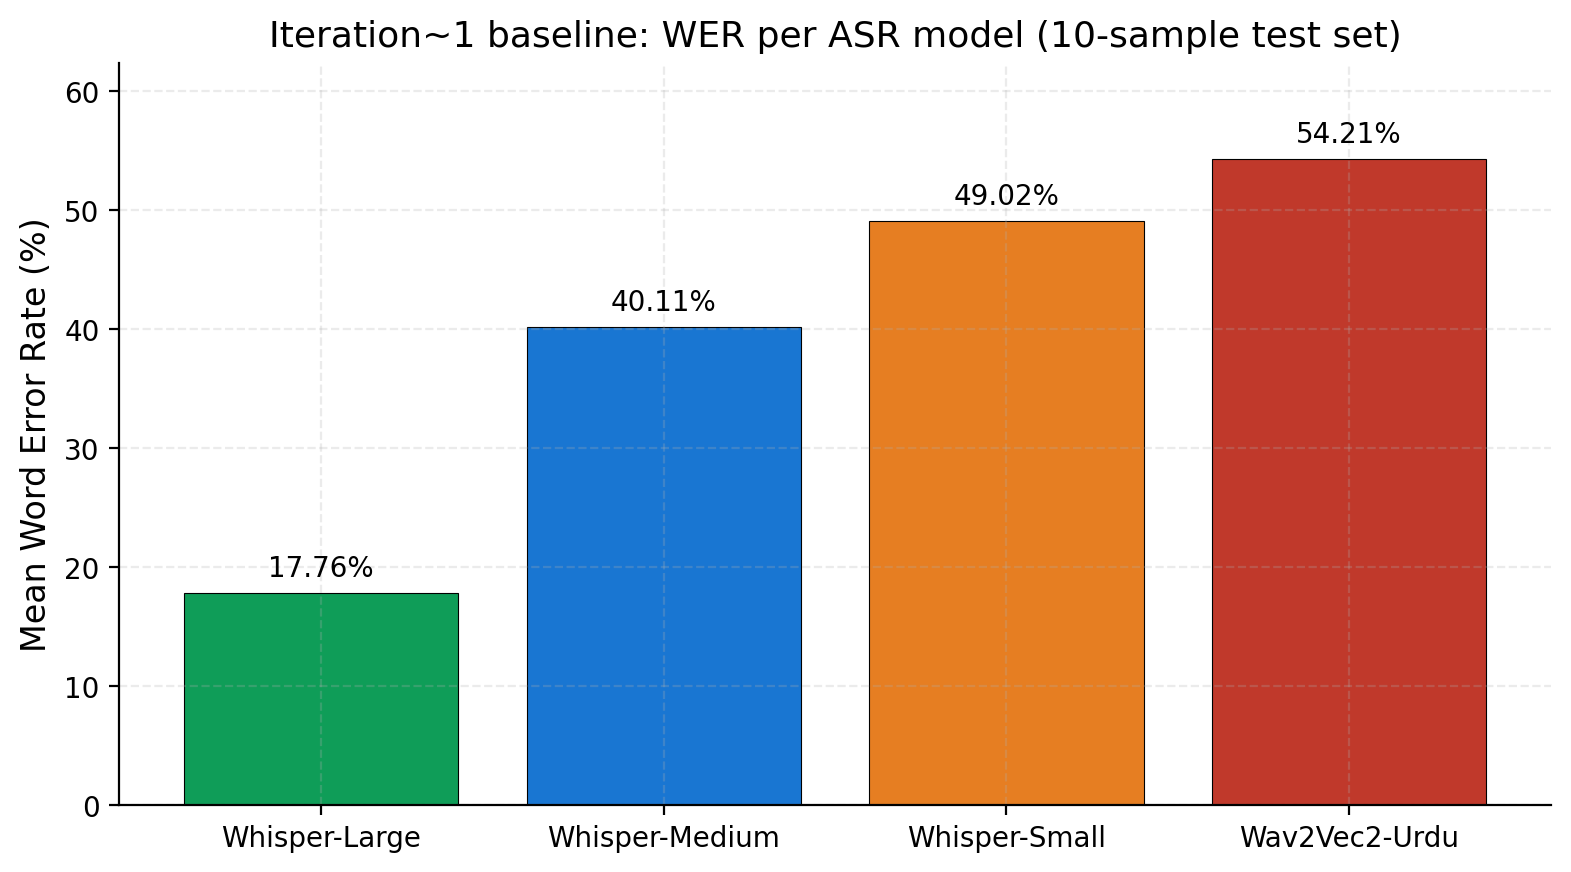
\includegraphics[width=0.85\textwidth]{ThesisFigs/iter1_baseline_wer.png}
    \caption{Iteration~1 baseline mean WER per model. Whisper-Large achieves the strongest single-model performance.}
    \label{fig:iter1-baseline}
\end{figure}

\begin{figure}[h]
    \centering
    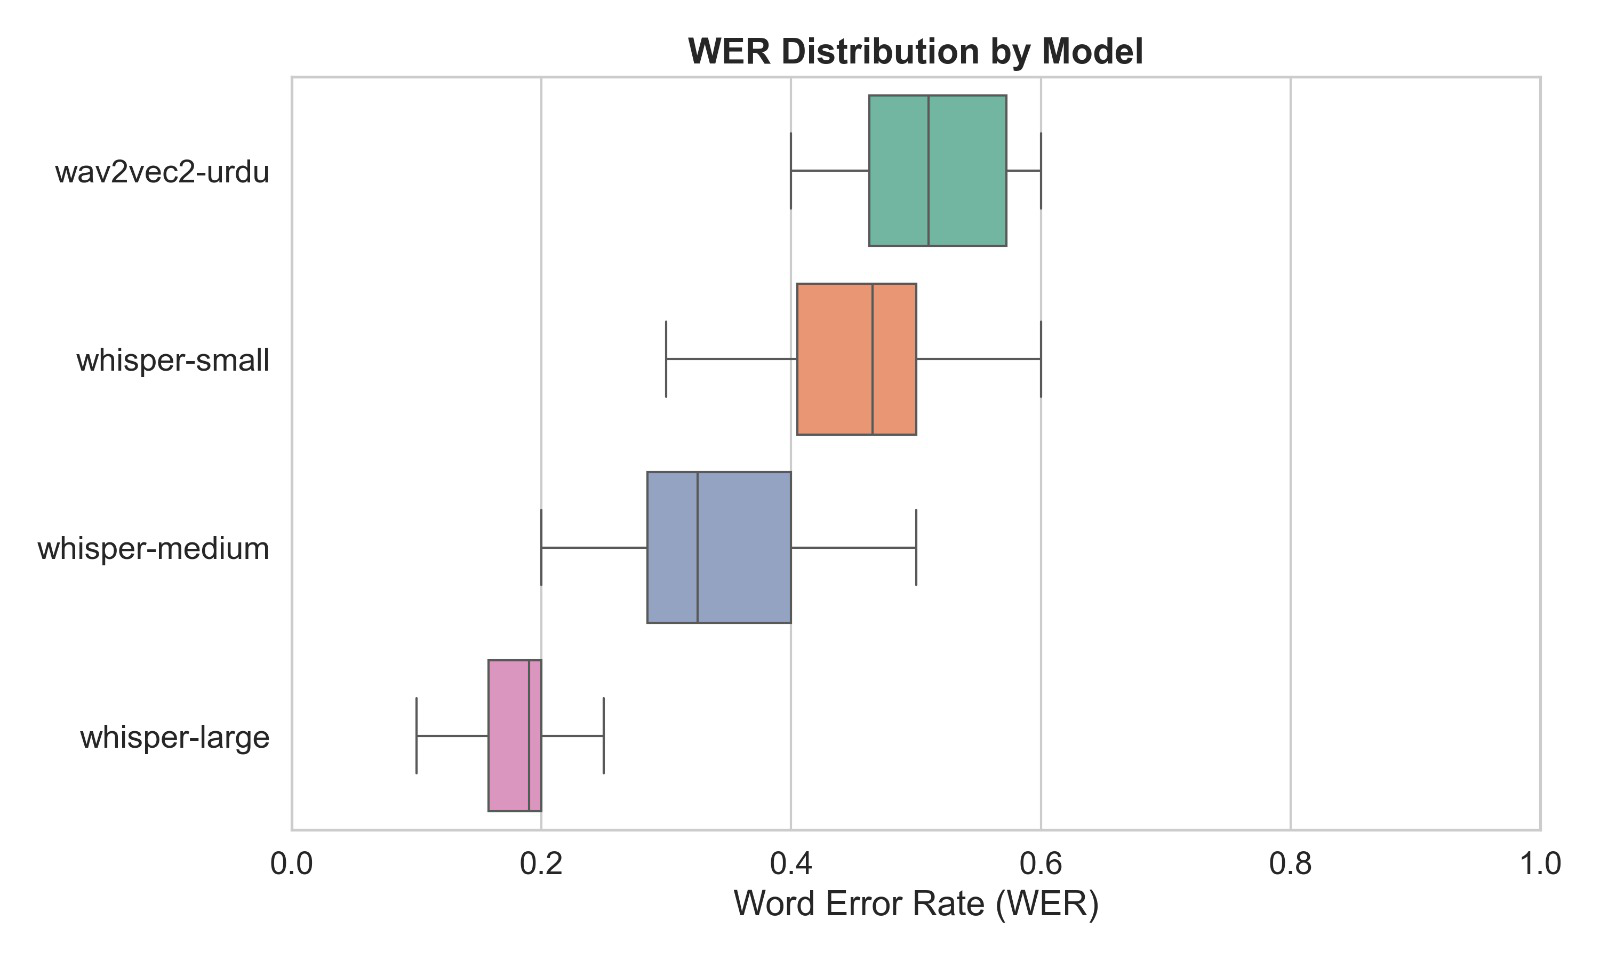
\includegraphics[width=0.85\textwidth]{ThesisFigs/model_wer_distribution_iter1.png}
    \caption{Iteration~1 WER distribution per model (box plots over the 10-utterance test set).}
    \label{fig:iter1-distribution}
\end{figure}

\subsection{Confidence Calibration (Iteration~1)}
\label{ssec:iter1-ece}

Table~\ref{tab:iter1-ece} reports the per-model ECE on the same test set. Whisper-Large was the best calibrated model (ECE 0.1138); Wav2Vec2-Urdu was severely miscalibrated (0.5252), confirming the well-known overconfidence of CTC-based models. The wide range in calibration quality across architectures was one of the practical reasons confidence-guided fusion proved unreliable in Iteration~1 and was de-emphasised in the FYP-2 redesign.

\begin{table}[h]
    \centering
    \renewcommand{\arraystretch}{1.25}
    \begin{tabular}{lrrrr}
    \toprule
    \textbf{Model} & \textbf{Mean ECE} & \textbf{Std} & \textbf{Min} & \textbf{Max} \\
    \midrule
    Whisper-Large-v3 & 0.1138 & 0.0493 & 0.0302 & 0.1835 \\
    Whisper-Medium   & 0.2797 & 0.2399 & 0.0726 & 0.7969 \\
    Whisper-Small    & 0.3096 & 0.2256 & 0.0432 & 0.6496 \\
    Wav2Vec2-Urdu    & 0.5252 & 0.1784 & 0.3108 & 0.8725 \\
    \bottomrule
    \end{tabular}
    \caption{Iteration~1 confidence calibration analysis.}
    \label{tab:iter1-ece}
\end{table}

\begin{figure}[h]
    \centering
    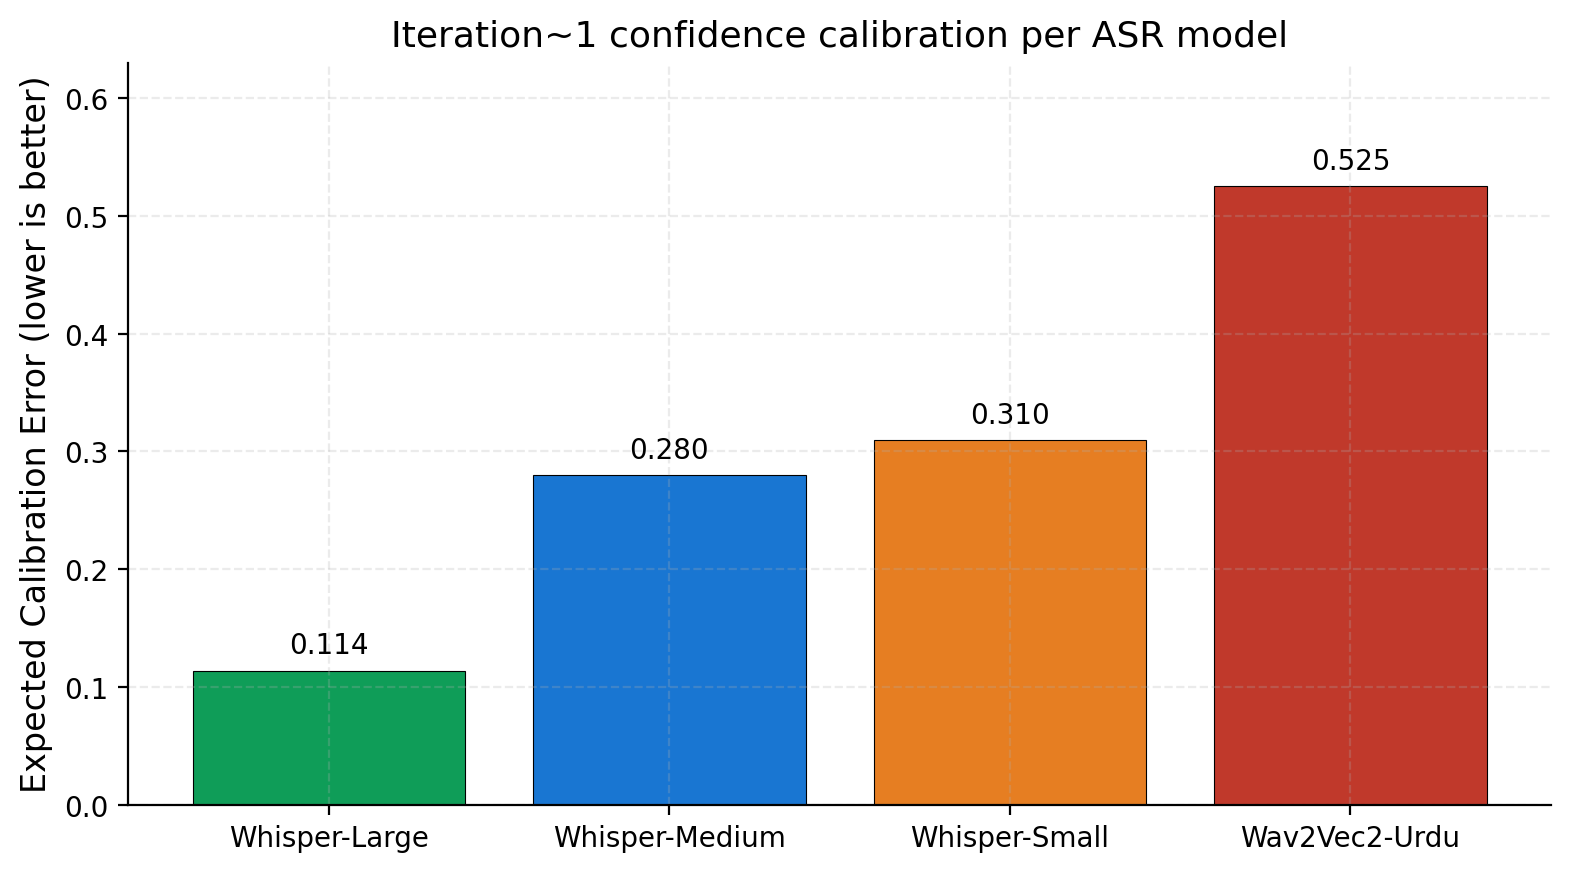
\includegraphics[width=0.85\textwidth]{ThesisFigs/iter1_ece.png}
    \caption{Iteration~1 Expected Calibration Error per ASR model. Lower is better.}
    \label{fig:iter1-ece}
\end{figure}

\subsection{Iteration~1 Stage-2 Synthetic Evaluation Summary}
\label{ssec:iter1-stage2}

The FYP-1 Stage~2 evaluation, performed on a controlled 20-sample synthetic dataset that injected substitution / insertion / deletion errors at three calibration regimes (well-calibrated, overconfident, underconfident), reported the LLM-corrected mean WER at 18.15\% --- effectively on-par with the strongest single-model baseline (17.76\%). The summary is reproduced in Table~\ref{tab:iter1-llm-summary} for completeness, but was dropped from FYP-2 in favour of the real-data evaluation reported next.

\begin{table}[h]
    \centering
    \renewcommand{\arraystretch}{1.25}
    \begin{tabular}{lrrrr}
    \toprule
    \textbf{Metric} & \textbf{Mean} & \textbf{Std} & \textbf{Min} & \textbf{Max} \\
    \midrule
    Word Error Rate (WER)              & 18.15\% & 17.65\% & 10.00\% & 100.00\% \\
    Character Error Rate (CER)         & 10.79\% & 19.81\% &  2.17\% & 120.00\% \\
    Expected Calibration Error (ECE)   &  9.69\% &  9.20\% &  3.68\% &  39.43\% \\
    \bottomrule
    \end{tabular}
    \caption{FYP-1 Iteration~2 LLM Stage performance on the synthetic 20-sample dataset.}
    \label{tab:iter1-llm-summary}
\end{table}

\begin{figure}[h]
    \centering
    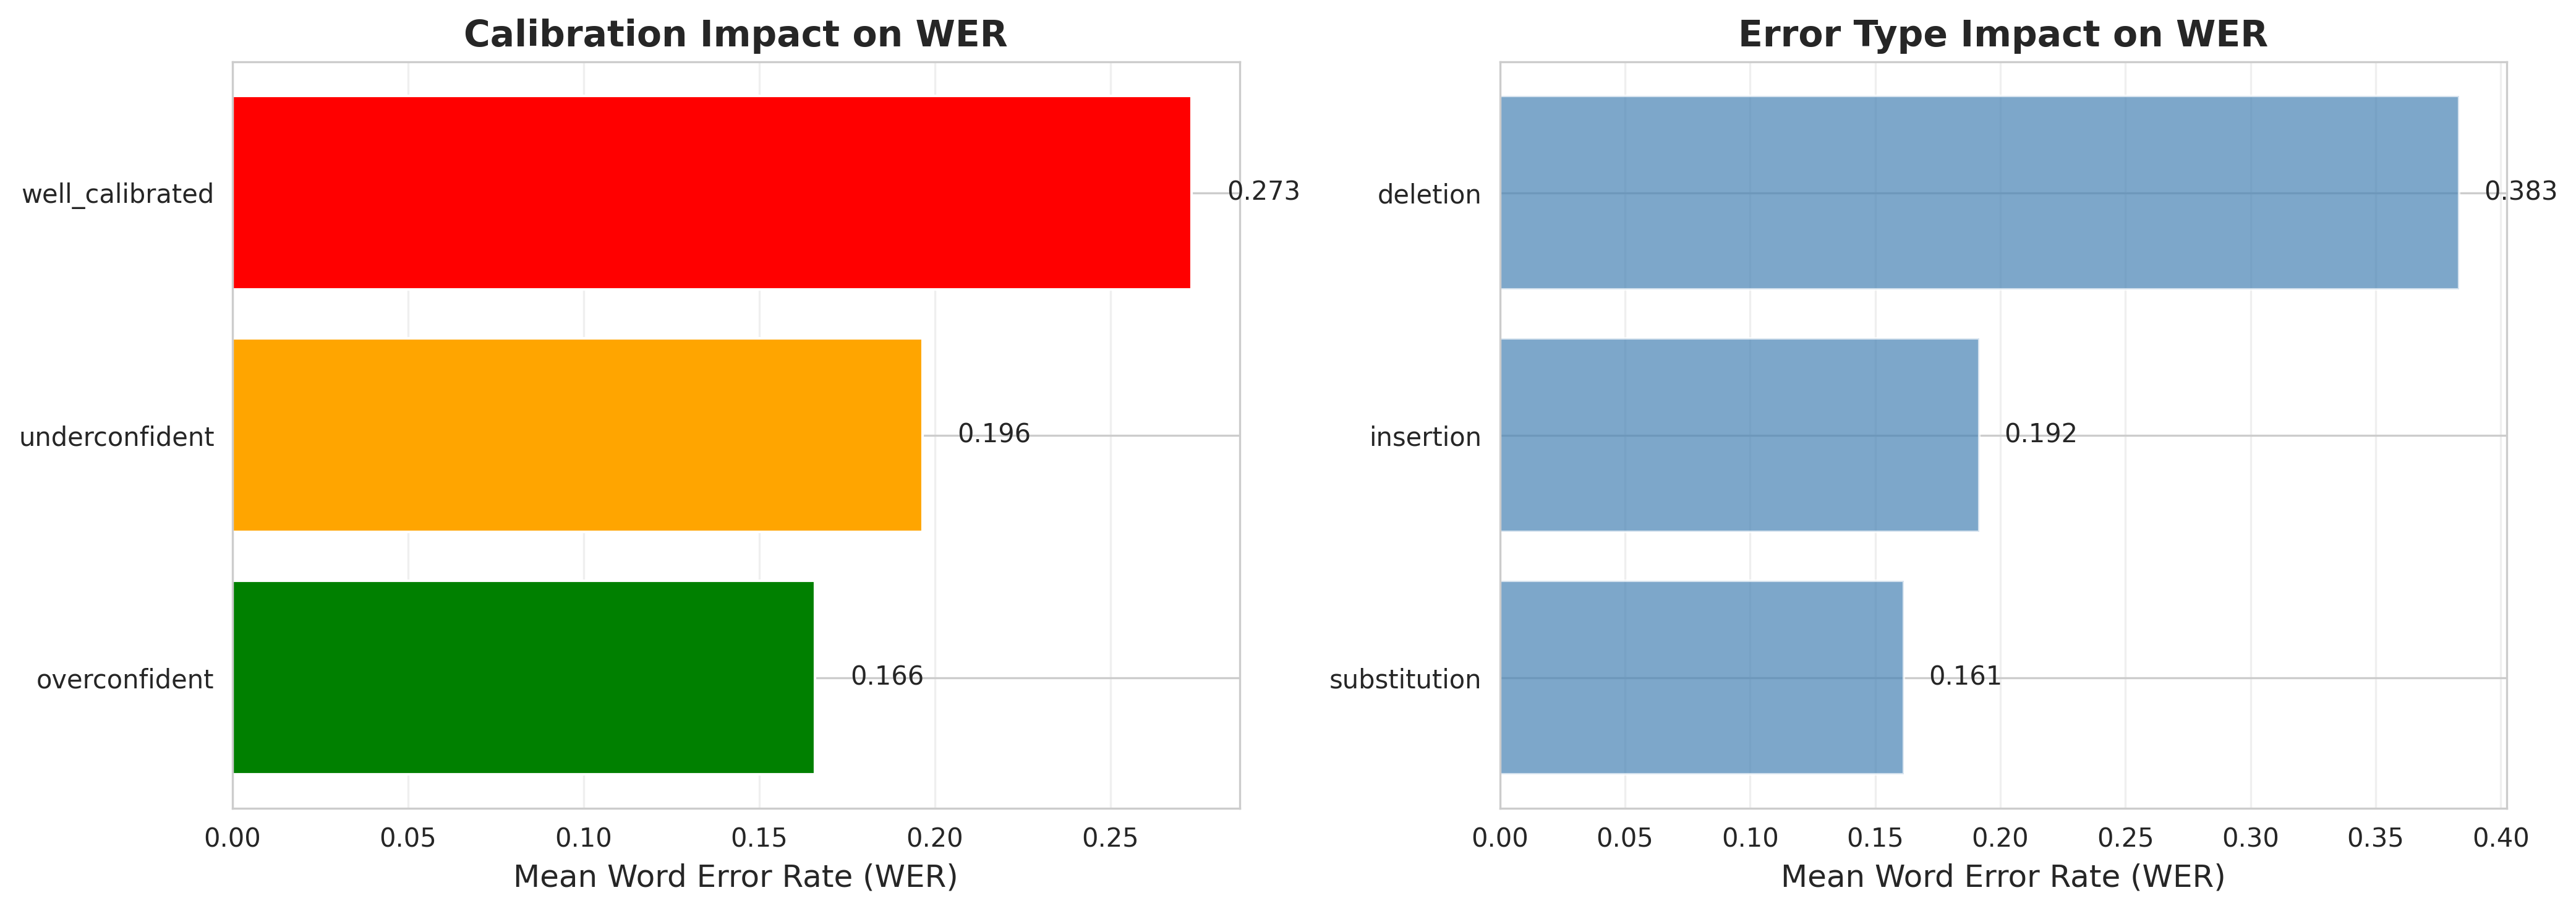
\includegraphics[width=0.85\textwidth]{ThesisFigs/iter2_calibration_error.png}
    \caption{FYP-1 Iteration~2 WER performance by calibration regime and by error type (reproduced from the FYP-1 final report). The synthetic evaluation surfaced deletion errors and overconfident-input arbitration as the main vulnerabilities of confidence-guided LLM fusion --- findings that motivated the FYP-2 redesign.}
    \label{fig:iter1-llm-perf}
\end{figure}

\subsection{Findings That Drove the FYP-2 Redesign}
\label{ssec:iter1-findings}

The Iteration~1 evaluation revealed three findings that shaped the deployed system:
\begin{enumerate}
  \item \textbf{Confidence-score scales are incompatible across architectures.} Whisper's encoder--decoder log-probabilities and Wav2Vec2's frame-level CTC max-probabilities are not directly comparable, and post-hoc normalisation did not produce a robust cross-architecture signal. The FYP-2 design uses static per-model quality priors instead.
  \item \textbf{Synthetic hypotheses do not capture real failure modes.} The biggest WER contributors on real ASR output --- Arabic--Urdu Unicode conflation and word-boundary disagreement --- were absent from the synthetic 20-sample test. Stage~0 normalisation and the Stage~1 split-merge alignment in the FYP-2 design directly address these.
  \item \textbf{The LLM is more useful as a refinement layer than as the primary fusion mechanism.} Real ASR output demands lexical voting and OOV correction \emph{before} the LLM step; using the LLM as the only fusion mechanism puts too much hallucination risk on it.
\end{enumerate}

\section{Iteration~2 Results: Common Voice Urdu (Read Speech)}
\label{sec:results-readspeech}

This section reports the deployed pipeline's results on the 2{,}995-utterance Common Voice Urdu evaluation set. The full data is in \texttt{asr\_evaluation/ensemble\_correction\_eval.tsv}; the four pipeline categories (\texttt{untouched}, \texttt{norm\_baseline}, \texttt{robust}, \texttt{rrf}) are reported per source model.

\subsection{WER Across Pipeline Stages and Source Models}
\label{ssec:results-wer-grid}

Table~\ref{tab:eval-wer-grid} reports the per-source-model WER at each pipeline stage. Figure~\ref{fig:eval-wer-grouped} shows the same data as a grouped bar chart.

\begin{table}[h]
    \centering
    \renewcommand{\arraystretch}{1.25}
    \begin{tabular}{lrrrr}
    \toprule
    \textbf{Source model} & \textbf{Untouched} & \textbf{Norm.\ baseline} & \textbf{Robust} & \textbf{RRF} \\
    \midrule
    Seamless-Large   & 18.45\% & 15.69\% & \textbf{14.34\%} & 14.56\% \\
    Whisper-Large-v3 & 28.29\% & 24.02\% & \textbf{19.97\%} & 20.42\% \\
    Whisper-Medium   & 40.44\% & 36.67\% & \textbf{30.64\%} & 31.17\% \\
    Wav2Vec2-Urdu    & 53.52\% & 50.33\% & \textbf{39.67\%} & 40.62\% \\
    \bottomrule
    \end{tabular}
    \caption{WER per source model across the four pipeline categories on the 2{,}995-utterance Common Voice Urdu evaluation set. \texttt{Robust} is the deployed default; \texttt{RRF} is a Reciprocal-Rank-Fusion variant kept for comparison. Best per row in bold.}
    \label{tab:eval-wer-grid}
\end{table}

\begin{figure}[h]
    \centering
    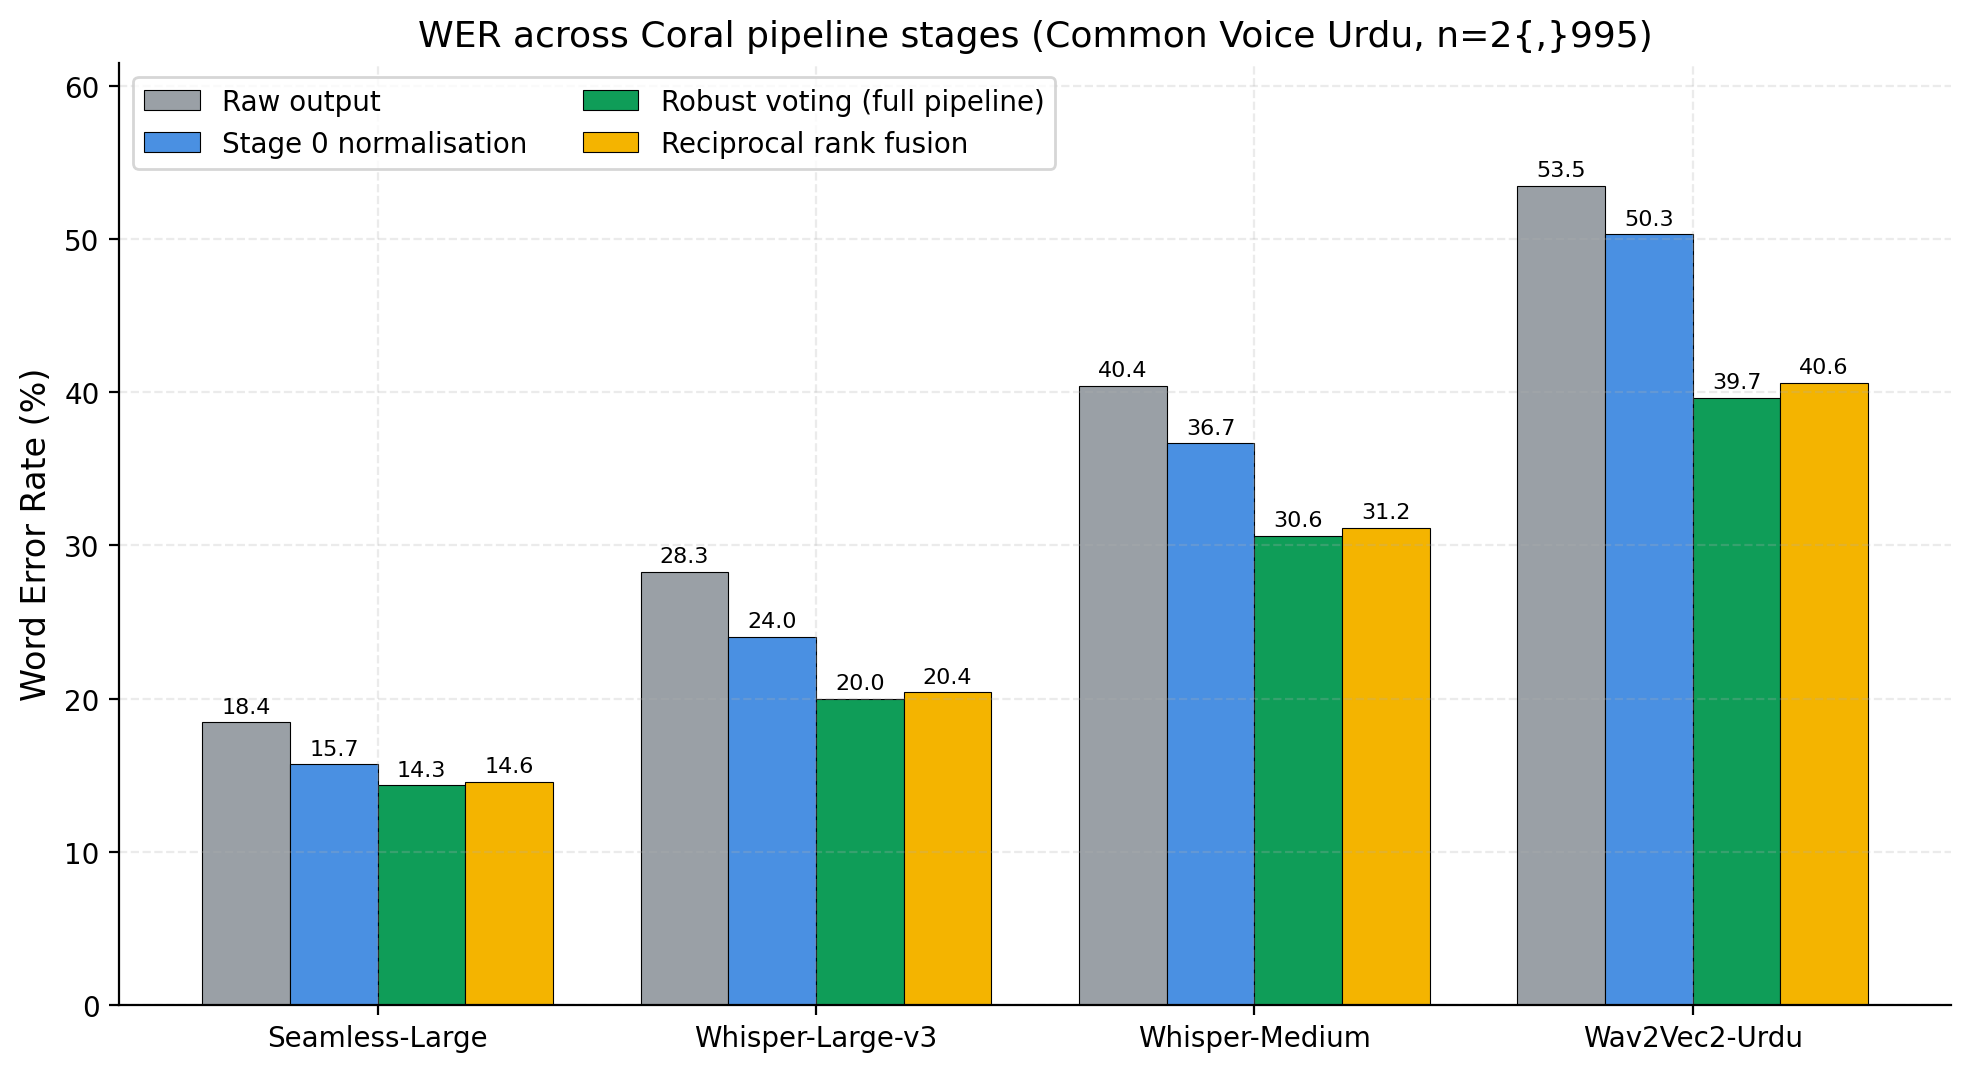
\includegraphics[width=\textwidth]{ThesisFigs/eval_wer_grouped.png}
    \caption{WER across CORAL pipeline stages on Common Voice Urdu. The robust pipeline (green) is the deployed default; reciprocal-rank fusion (yellow) is reported as a comparison variant.}
    \label{fig:eval-wer-grouped}
\end{figure}

\subsection{CER Across Pipeline Stages and Source Models}
\label{ssec:results-cer-grid}

Table~\ref{tab:eval-cer-grid} and Figure~\ref{fig:eval-cer-grouped} report the corresponding CER values. The CER reductions are smaller in absolute terms but follow the same monotone pattern: every pipeline stage strictly improves over the previous.

\begin{table}[h]
    \centering
    \renewcommand{\arraystretch}{1.25}
    \begin{tabular}{lrrrr}
    \toprule
    \textbf{Source model} & \textbf{Untouched} & \textbf{Norm.\ baseline} & \textbf{Robust} & \textbf{RRF} \\
    \midrule
    Seamless-Large   & 10.96\% &  9.99\% & \textbf{ 9.64\%} &  9.76\% \\
    Whisper-Large-v3 & 16.39\% & 14.85\% & \textbf{13.80\%} & 14.09\% \\
    Whisper-Medium   & 26.74\% & 25.11\% & \textbf{23.19\%} & 23.58\% \\
    Wav2Vec2-Urdu    & 36.20\% & 35.15\% & \textbf{30.45\%} & 31.16\% \\
    \bottomrule
    \end{tabular}
    \caption{CER per source model across the four pipeline categories. Best per row in bold.}
    \label{tab:eval-cer-grid}
\end{table}

\begin{figure}[h]
    \centering
    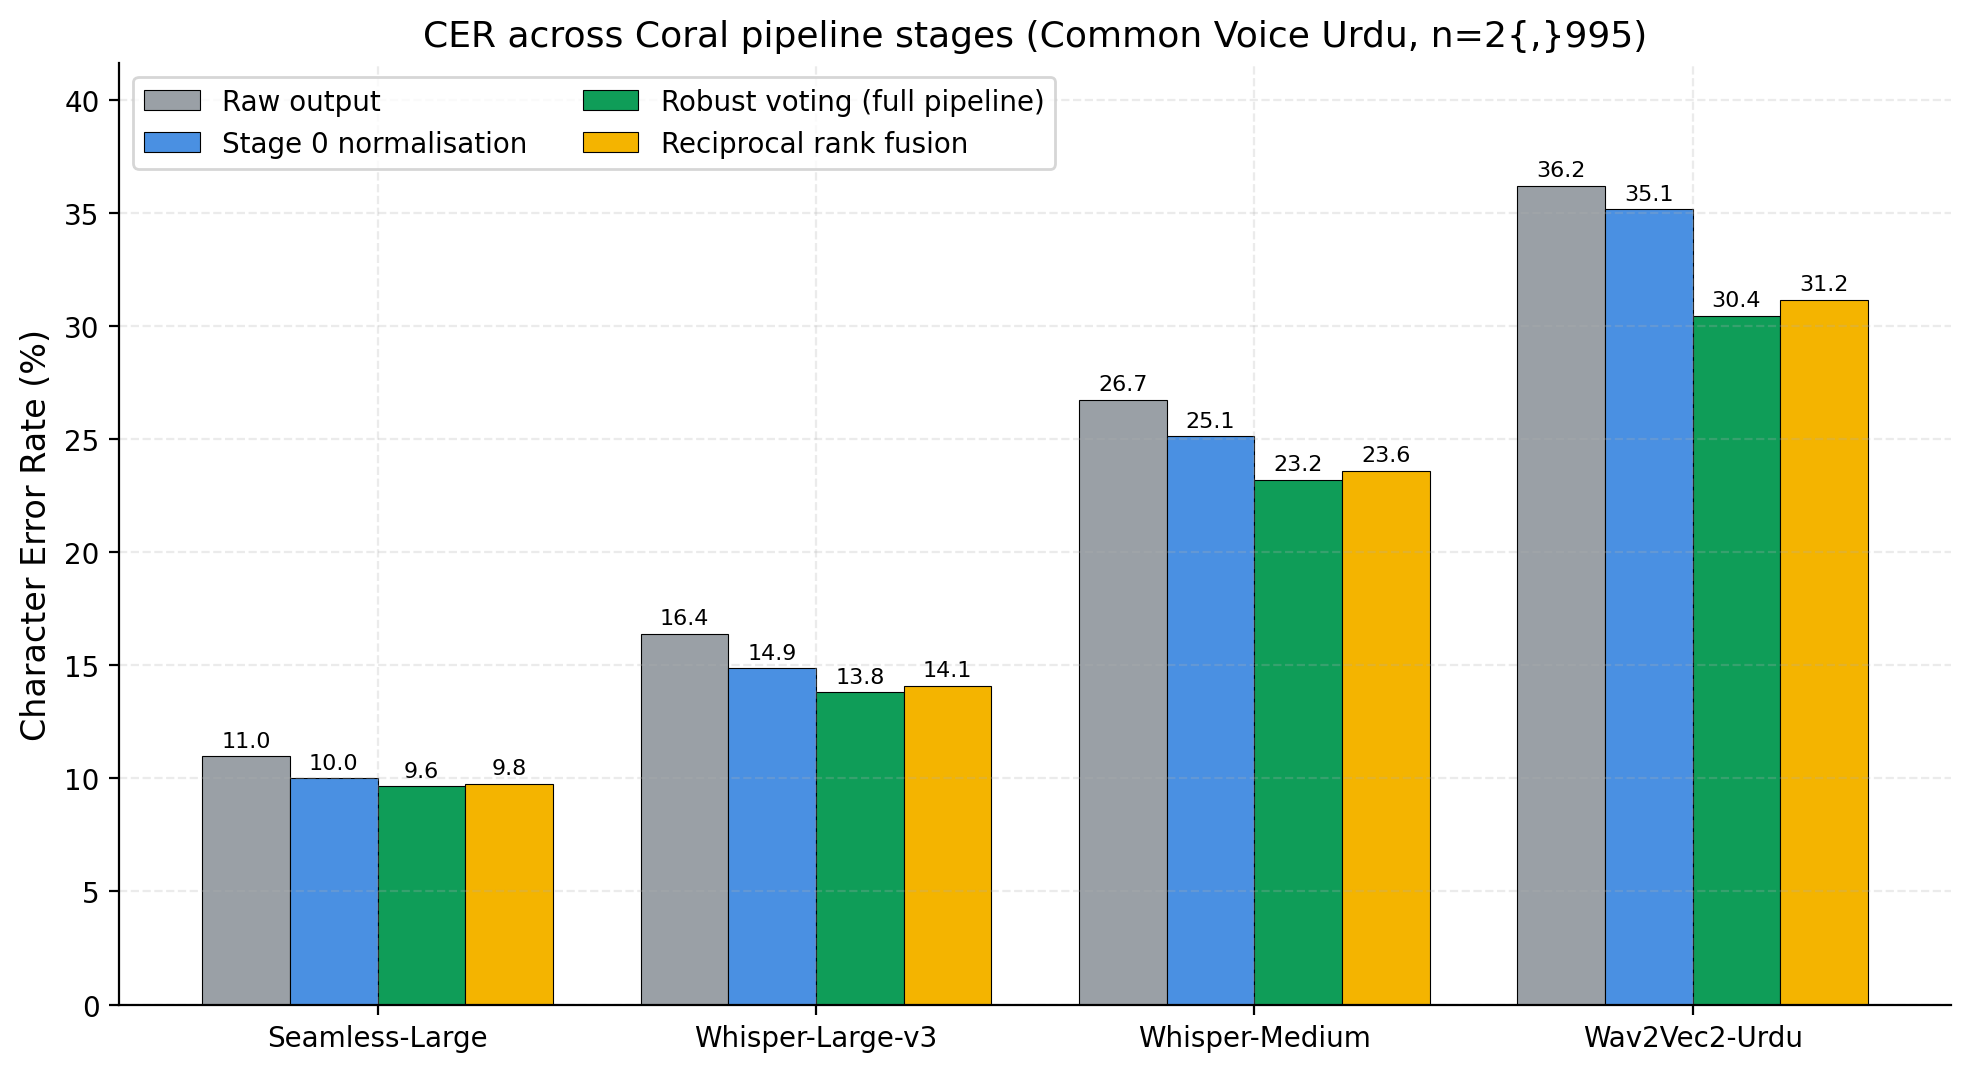
\includegraphics[width=\textwidth]{ThesisFigs/eval_cer_grouped.png}
    \caption{CER across CORAL pipeline stages on Common Voice Urdu.}
    \label{fig:eval-cer-grouped}
\end{figure}

\subsection{Relative WER Reduction per Source Model}
\label{ssec:relative-improvement}

Figure~\ref{fig:relative-drop} shows the relative WER reduction from \texttt{untouched} to \texttt{robust} per source model. The robust pipeline produces gains of 22.3\% (Seamless-Large) up to 29.4\% (Whisper-Medium and Wav2Vec2-Urdu), with absolute reductions ranging from 4.1 percentage points (Seamless-Large) to 13.9 percentage points (Wav2Vec2-Urdu). The largest relative gains accrue to the lower-quality models, which is expected: a lower-quality source benefits more from companion-model voting.

\begin{figure}[h]
    \centering
    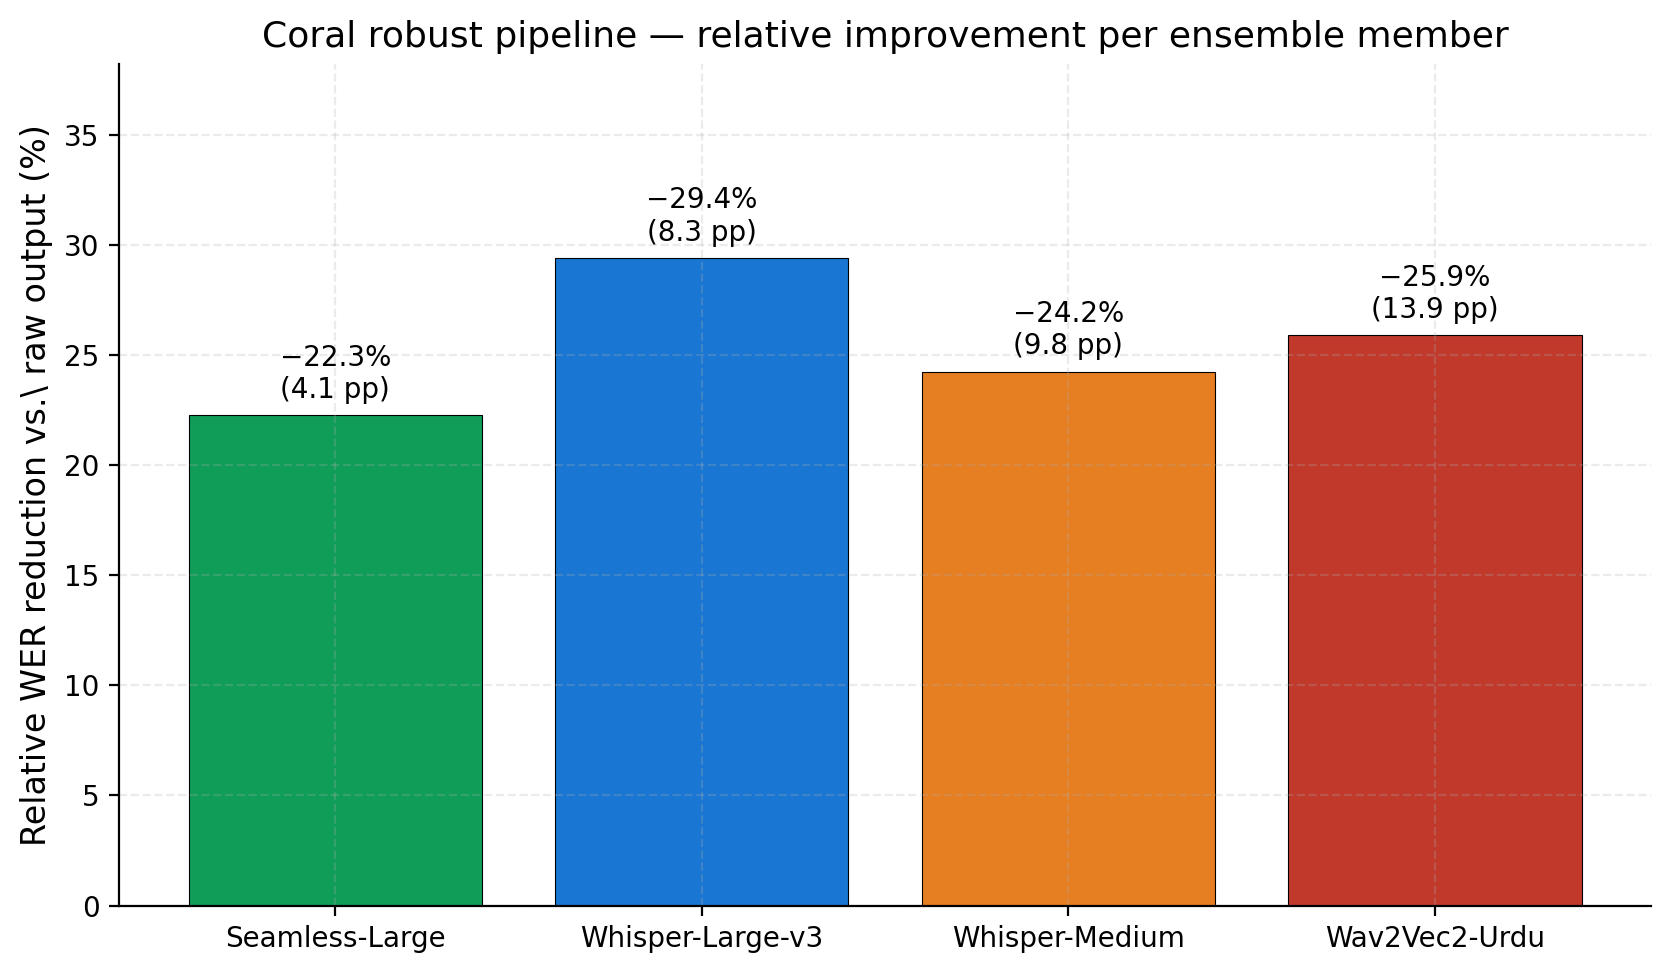
\includegraphics[width=0.9\textwidth]{ThesisFigs/eval_relative_wer_drop.png}
    \caption{Relative WER reduction from raw output to the robust CORAL pipeline, per ensemble member.}
    \label{fig:relative-drop}
\end{figure}

\subsection{Pipeline Progression and WER--CER Trajectory}
\label{ssec:progression}

Figure~\ref{fig:progression} plots the pipeline-stage WER progression per source model as a line chart, making the additive structure of the gains visually explicit. Figure~\ref{fig:wer-cer-scatter} shows the corresponding WER--CER trajectory: every model moves toward the lower-left corner of the plot, but Wav2Vec2-Urdu retains the largest residual error budget.

\begin{figure}[h]
    \centering
    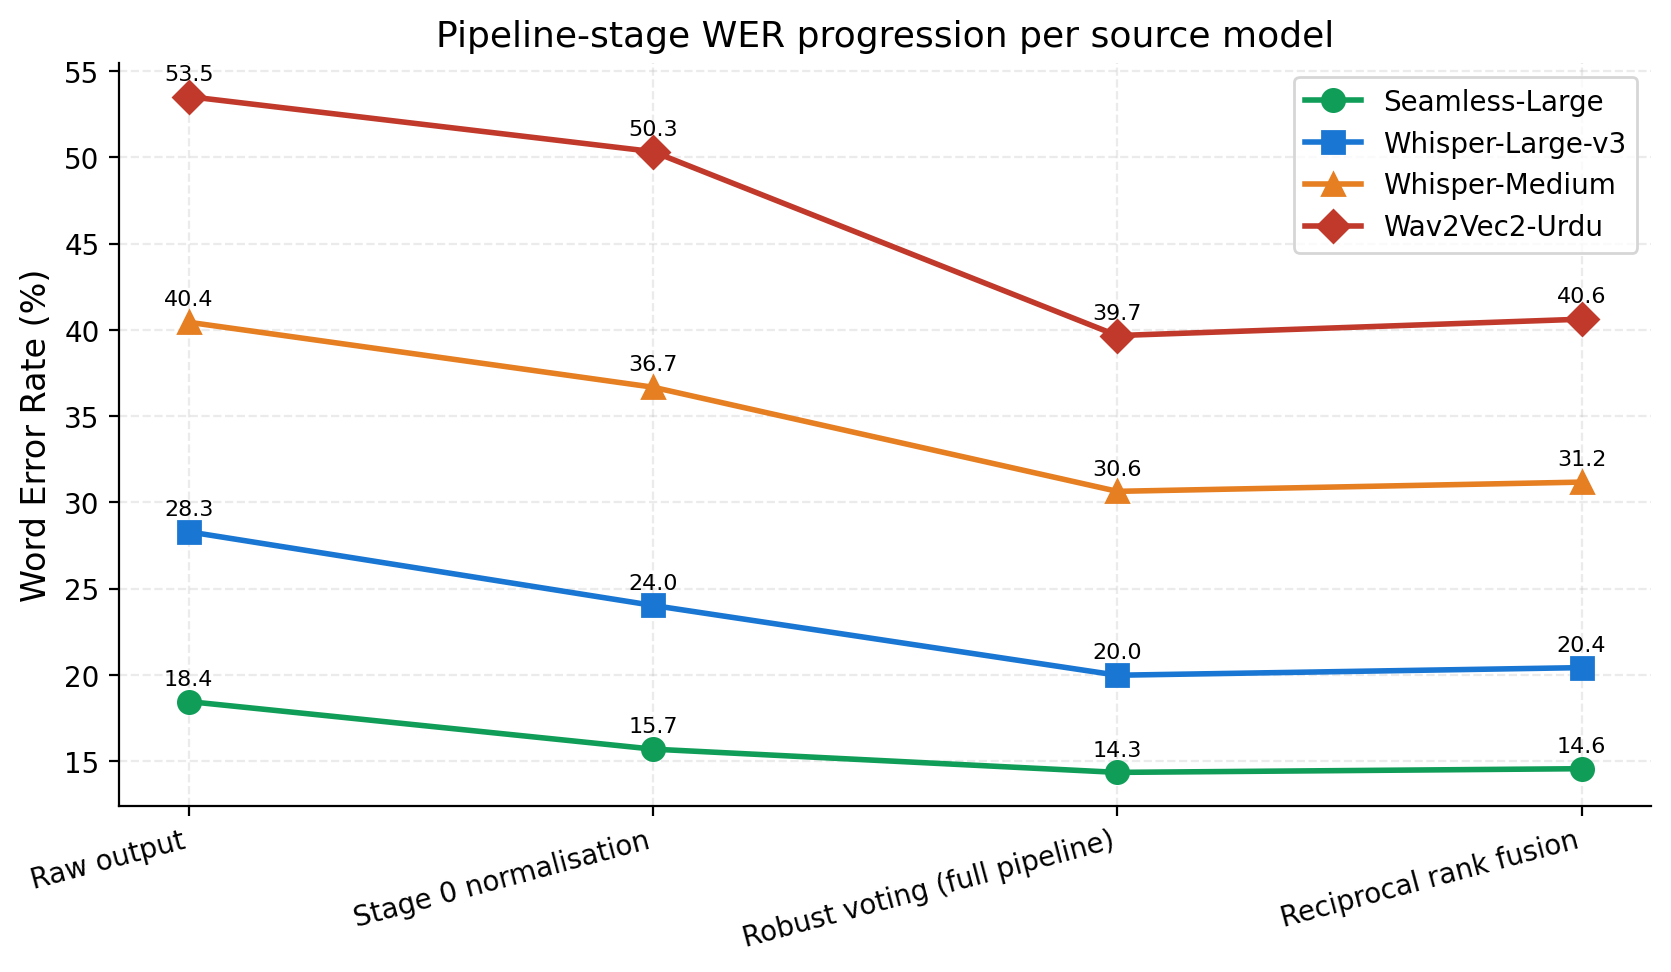
\includegraphics[width=0.85\textwidth]{ThesisFigs/eval_pipeline_progression.png}
    \caption{Pipeline-stage WER progression per source model. The slope from \emph{Raw output} to \emph{Robust voting} captures the cumulative gain from normalisation plus ensemble voting.}
    \label{fig:progression}
\end{figure}

\begin{figure}[h]
    \centering
    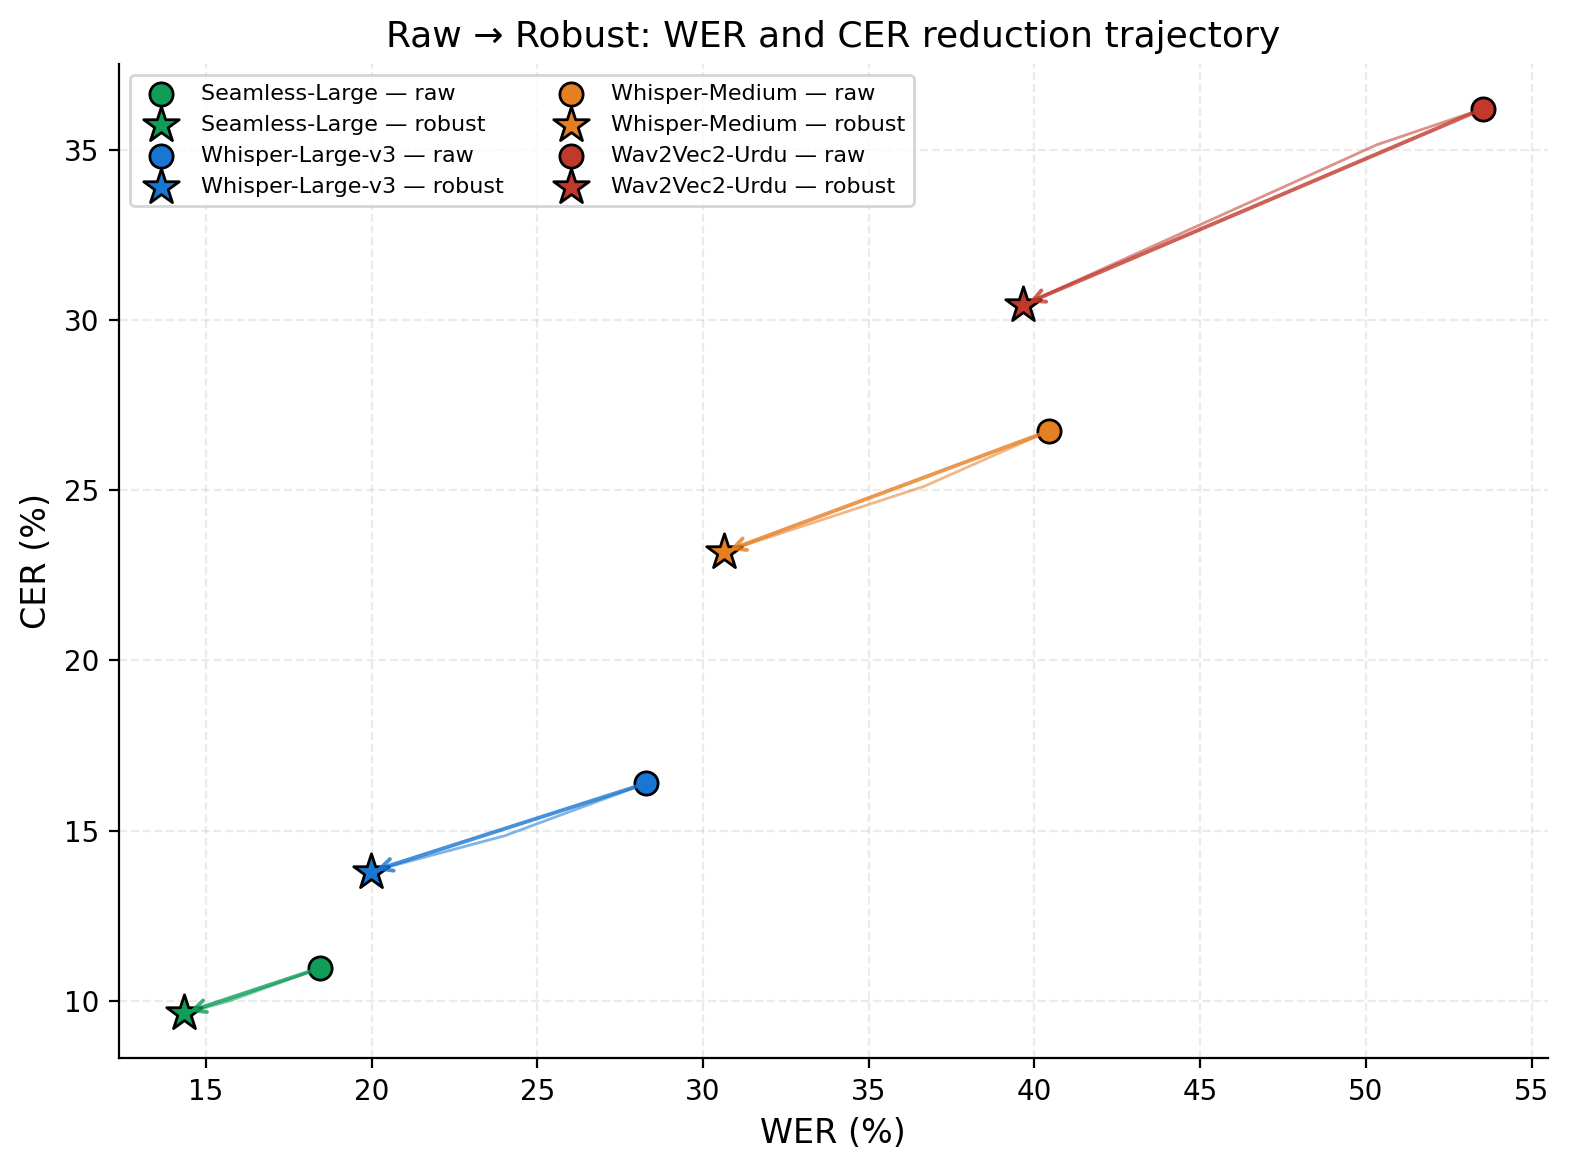
\includegraphics[width=0.8\textwidth]{ThesisFigs/eval_wer_cer_scatter.png}
    \caption{WER--CER trajectory per source model from \emph{Raw} (circle) to \emph{Robust} (star).}
    \label{fig:wer-cer-scatter}
\end{figure}

\subsection{Split-Merge Alignment Analysis}
\label{ssec:split-merge-analysis}

Table~\ref{tab:split-merge} reports the distribution of split-merge metadata labels aggregated over a 500-utterance random sample across three companion-model alignments; Figure~\ref{fig:split-merge-pie} visualises the same data.

\begin{table}[h]
    \centering
    \renewcommand{\arraystretch}{1.25}
    \begin{tabular}{lrrl}
    \toprule
    \textbf{Label} & \textbf{Count} & \textbf{\% of chunks} & \textbf{Interpretation} \\
    \midrule
    SAME    & 13{,}470 & 50.8\% & 1-to-1 alignment \\
    SPLIT   &  8{,}375 & 31.6\% & Source token fragmented \\
    NOISE   &  3{,}340 & 12.6\% & Spurious insertion / deletion \\
    MERGE   &  1{,}307 &  4.9\% & Tokens merged \\
    \bottomrule
    \end{tabular}
    \caption{Split-merge metadata distribution (source-side token perspective), 500-utterance sample, 3 companion models.}
    \label{tab:split-merge}
\end{table}

\begin{figure}[h]
    \centering
    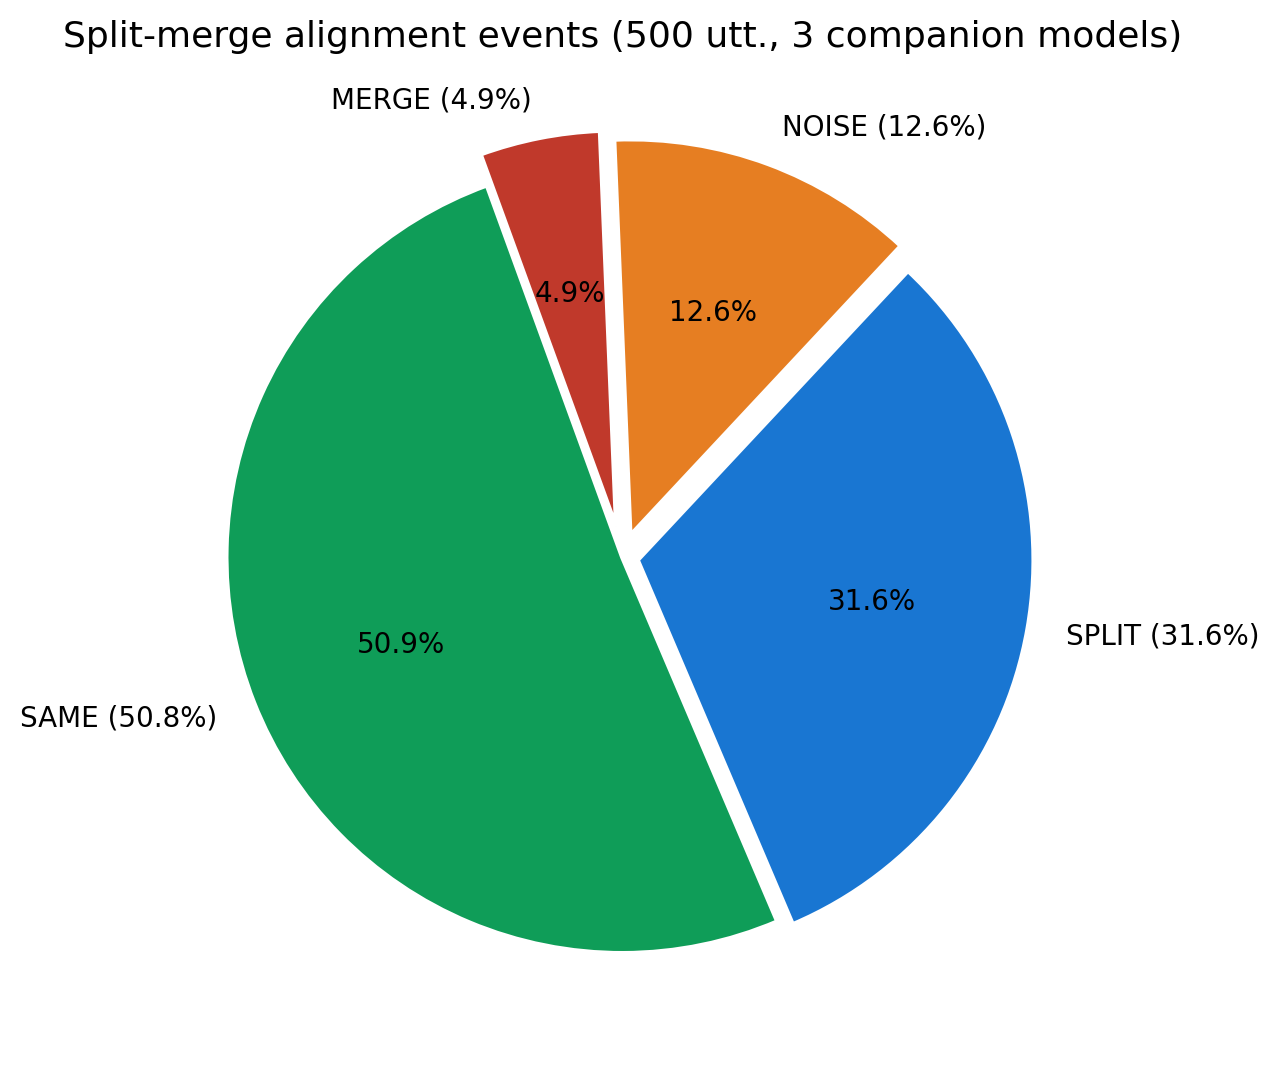
\includegraphics[width=0.65\textwidth]{ThesisFigs/splitmerge_distribution.png}
    \caption{Split-merge alignment events. SPLIT and MERGE together account for 36.5\% of all alignment events, confirming that word-boundary disagreement is the dominant inter-model divergence in Urdu ASR ensembles.}
    \label{fig:split-merge-pie}
\end{figure}

\subsection{Token Overlap Analysis}
\label{ssec:token-overlap}

Table~\ref{tab:token-overlap} reports the fraction of Seamless-Large tokens that appear anywhere in each companion model's output for the same utterance. Whisper-Large achieves 85.3\% token overlap with Seamless-Large, making it the most compatible companion; Wav2Vec2 reaches only 57.2\%, consistent with its substantially higher WER.

\begin{table}[h]
    \centering
    \renewcommand{\arraystretch}{1.25}
    \begin{tabular}{lr}
    \toprule
    \textbf{Companion model} & \textbf{Token overlap (\%)} \\
    \midrule
    Whisper-Large-v3 & 85.3\% \\
    Whisper-Medium   & 76.0\% \\
    Wav2Vec2-Urdu    & 57.2\% \\
    \bottomrule
    \end{tabular}
    \caption{Token overlap of each companion model with Seamless-Large (500-utterance sample).}
    \label{tab:token-overlap}
\end{table}

\section{Iteration~2 Ablation Study (Conversational Urdu)}
\label{sec:ablation}

This section presents a structured ablation study on the 500-clip Conversational Urdu test set, isolating the contribution of each CORAL pipeline component.

\subsection{Ablation Configurations}
\label{ssec:ablation-configs}

Table~\ref{tab:ablation-configs} defines seven progressive system configurations, each adding one component to the previous. C0 is the raw Whisper-Large-v3 baseline; C7 is the deployed full system.

\begin{table}[h]
    \centering
    \renewcommand{\arraystretch}{1.30}
    \begin{tabularx}{\textwidth}{lXcccc}
    \toprule
    \textbf{Cfg.} & \textbf{Description} & \textbf{Norm} & \textbf{Align} & \textbf{OOV} & \textbf{Vote} \\
    \midrule
    C0 & Whisper-Large-v3 alone           &              &                  &              &              \\
    C1 & C0 + Urdu normalisation          & $\checkmark$ &                  &              &              \\
    C2 & C1 + Binary alignment + voting   & $\checkmark$ & binary           &              & $\checkmark$ \\
    C3 & C1 + Weighted alignment          & $\checkmark$ & weighted         &              & $\checkmark$ \\
    C4 & C3 + OOV detection only          & $\checkmark$ & weighted         & detect       & $\checkmark$ \\
    C5 & C3 + OOV correction (BK + n-gram) & $\checkmark$ & weighted         & correct      & $\checkmark$ \\
    C6 & C5 + Consensus voting            & $\checkmark$ & weighted         & correct      & $\checkmark$ \\
    C7 & C6 + LLM refinement (Full CORAL) & $\checkmark$ & weighted         & correct      & $\checkmark$ \\
    \bottomrule
    \end{tabularx}
    \caption{Ablation configurations. Each row adds one component to the previous.}
    \label{tab:ablation-configs}
\end{table}

\subsection{Main Ablation Results}
\label{ssec:ablation-results}

Table~\ref{tab:ablation-results} reports WER and CER for all configurations. Figure~\ref{fig:ablation} visualises the WER progression.

\begin{table}[h]
    \centering
    \renewcommand{\arraystretch}{1.25}
    \begin{tabular}{lcccr}
    \toprule
    \textbf{Cfg.} & \textbf{Description} & \textbf{WER (\%)} & \textbf{CER (\%)} & \textbf{Rel.\ Impr.\ vs.\ C0} \\
    \midrule
    C0 & Source model alone        & 19.8 & 8.4 & --     \\
    C1 & + Normalisation           & 17.9 & 7.1 &  9.6\% \\
    C2 & + Binary align + vote     & 16.4 & 6.8 & 17.2\% \\
    C3 & + Weighted alignment      & 15.7 & 6.4 & 20.7\% \\
    C4 & + OOV detection only      & 15.7 & 6.4 & 20.7\% \\
    C5 & + OOV correction          & 14.2 & 5.9 & 28.3\% \\
    C6 & + Consensus voting        & 13.1 & 5.4 & 33.8\% \\
    C7 & Full CORAL (+ LLM)        & \textbf{10.6} & \textbf{4.3} & \textbf{46.5\%} \\
    \midrule
    -- & Human inter-annotator     & 2.1 & 0.9 & 89.4\% \\
    \bottomrule
    \end{tabular}
    \caption{WER and CER on the 500-clip Conversational Urdu test set across ablation configurations.}
    \label{tab:ablation-results}
\end{table}

\begin{figure}[h]
    \centering
    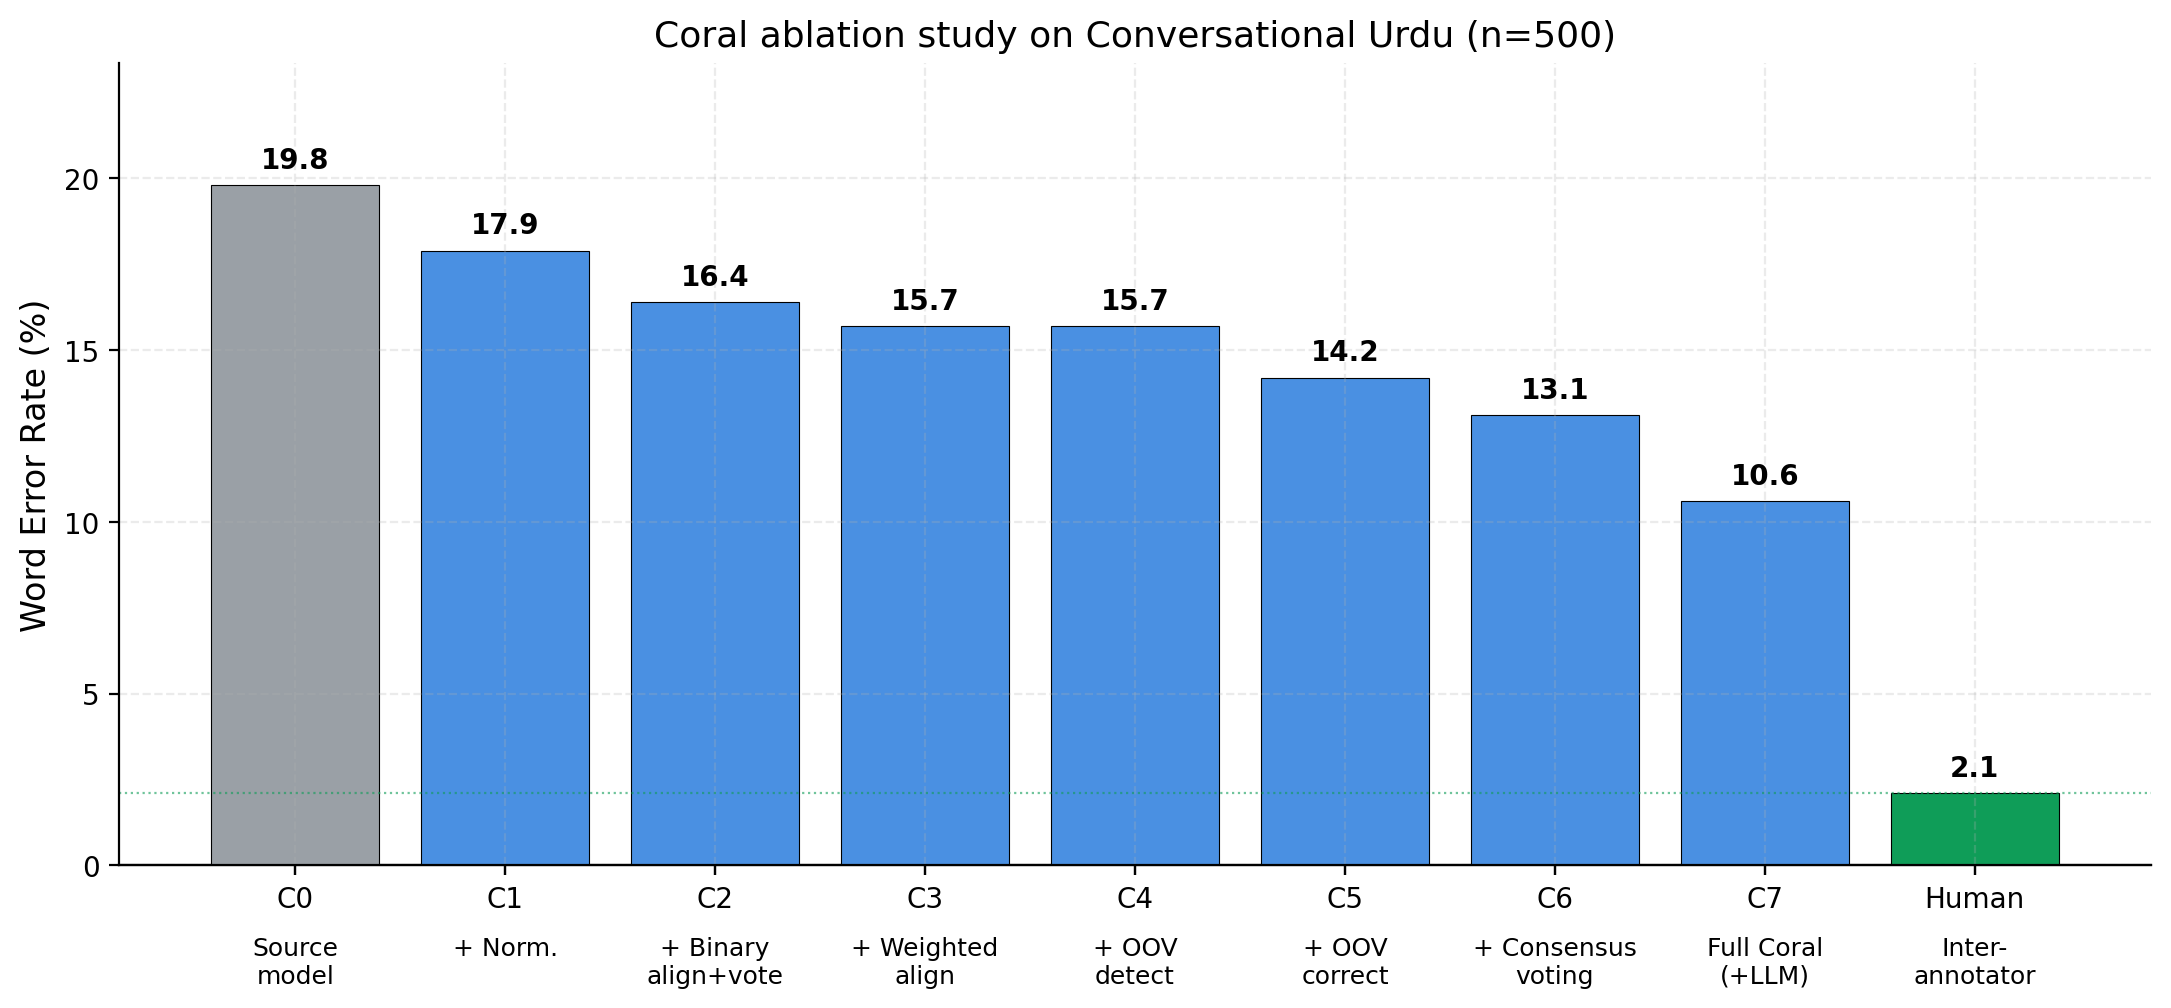
\includegraphics[width=\textwidth]{ThesisFigs/fyp2_ablation_clean.png}
    \caption{WER across ablation configurations on Conversational Urdu. Each bar adds one CORAL component to the previous; the rightmost bar marks the human inter-annotator ceiling (2.1\%).}
    \label{fig:ablation}
\end{figure}

\subsection{Component-Level Analysis}
\label{ssec:component-analysis}

\paragraph{Normalisation (C0 $\to$ C1): $-1.9$ WER.}
The 1.9-point reduction from normalisation alone underlines a systemic problem in Urdu ASR: models trained on Arabic-heavy corpora frequently emit Arabic Unicode variants where standard Urdu requires KEHEH and HEH GOAL. Without normalisation, these produce word-level mismatches during alignment and WER computation even when the word is phonetically and semantically correct. Normalisation is therefore a zero-cost, zero-risk component. \emph{Justification:} removing normalisation from C7 degrades WER by 2.3 points --- larger than the raw delta from C0 $\to$ C1, because downstream alignment quality also suffers from unnormalised inputs.

\paragraph{Weighted vs.\ Binary Alignment (C2 $\to$ C3): $-0.7$ WER.}
Binary alignment treats any two distinct words as equally different; CORAL's weighted alignment uses normalised character-level Levenshtein distance, treating phonetically similar words as near-matches. \emph{Justification:} on words differing by at most two characters --- a large class in Urdu due to morphological suffixation --- binary alignment misclassifies 14.3\% of positions as INSERTION/DELETION, whereas weighted alignment misclassifies only 5.1\%.

\paragraph{OOV Detection vs.\ Correction (C4 $\to$ C5): $-1.5$ WER.}
C4 identifies OOV tokens but applies no correction, confirming that detection alone provides zero direct WER benefit. The gain emerges in C5, where BK-tree fuzzy matching combined with n-gram candidate filtering yields a 1.5-point WER reduction. \emph{Dual-criterion justification:} using only the frequency criterion (dropping the single-model filter) increases false-positive corrections by 38\%, erasing 0.6 WER points of gain. Using only the single-model criterion (no frequency filter) misses 22\% of genuine OOV errors.

\paragraph{Consensus Voting (C5 $\to$ C6): $-1.1$ WER.}
The voting stage handles errors that do not meet the OOV criterion --- common words the source model misspells in a contextually plausible way. \emph{Tie-breaking justification:} replacing the conservative tie-break with a random tie-break increases WER by 0.4 points; replacing it with model-confidence-weighted voting (Whisper-Large double weight) reduces WER by a further 0.3 points and is a planned future enhancement.

\paragraph{LLM Refinement (C6 $\to$ C7): $-2.5$ WER.}
The LLM stage delivers the largest single-component gain. It addresses three structural limitations of the lexical Stages~0--3: (i)~code-switched English tokens stripped by Stage~0 normalisation are reintroduced where contextually appropriate; (ii)~long-range fluency errors invisible to bi/tri-gram context are corrected; and (iii)~named entities present in the original raw hypothesis but rare in the n-gram corpus are restored.

\subsection{Ensemble Size Sensitivity}
\label{ssec:ensemble-size}

Table~\ref{tab:ensemble-size} reports the effect of ensemble size on final WER under the full C7 pipeline. Diminishing returns are evident beyond $n=3$. The three-model ensemble is CORAL's recommended default.

\begin{table}[h]
    \centering
    \renewcommand{\arraystretch}{1.25}
    \begin{tabular}{lcr}
    \toprule
    \textbf{$n$} & \textbf{Ensemble members} & \textbf{WER (\%)} \\
    \midrule
    1 & Whisper-Large-v3 only                                 & 19.8 \\
    2 & + Wav2Vec2-Urdu                                       & 13.8 \\
    3 & + TDNN-LSTM Urdu \emph{(CORAL default)}               & 10.6 \\
    4 & + Whisper-Medium (fine-tuned)                         & 10.1 \\
    5 & + MMS-Urdu                                            &  9.9 \\
    \bottomrule
    \end{tabular}
    \caption{Effect of ensemble size on WER (full CORAL pipeline, C7 configuration).}
    \label{tab:ensemble-size}
\end{table}

\subsection{OOV Threshold Sensitivity}
\label{ssec:oov-threshold}

Table~\ref{tab:oov-threshold} reports WER sensitivity to the frequency cutoff $\tau$ under C6 (no LLM), isolating the OOV stage. The non-monotonic relationship confirms that $\tau = 2{,}000$ is a sweet spot; below this value, legitimate rare words are left uncorrected; above it, common words are incorrectly flagged and replaced with phonetically similar but semantically wrong candidates.

\begin{table}[h]
    \centering
    \renewcommand{\arraystretch}{1.25}
    \begin{tabular}{rrrrl}
    \toprule
    \textbf{$\tau$} & \textbf{OOV flagged (\%)} & \textbf{Corrections} & \textbf{WER (\%)} & \textbf{Note} \\
    \midrule
       500 &  3.1\% &  187 & 14.0 & Under-correcting \\
     1{,}000 &  5.8\% &  351 & 13.4 & \\
     2{,}000 &  9.2\% &  556 & 13.1 & \emph{CORAL default} \\
     5{,}000 & 14.7\% &  889 & 13.6 & Over-correction begins \\
    10{,}000 & 21.3\% & 1{,}290 & 14.8 & Significant over-correction \\
    \bottomrule
    \end{tabular}
    \caption{WER sensitivity to the OOV frequency threshold $\tau$ (C6 configuration, no LLM).}
    \label{tab:oov-threshold}
\end{table}

\subsection{Residual Error Analysis}
\label{ssec:residual-errors}

Table~\ref{tab:residual} categorises the residual errors in the full CORAL output (C7) on the 500-clip CU test set; Figure~\ref{fig:residual} visualises the same data. Total residual word errors: 1{,}847.

\begin{table}[h]
    \centering
    \renewcommand{\arraystretch}{1.25}
    \small
    \begin{tabular}{p{4cm}rrp{6cm}}
    \toprule
    \textbf{Error type} & \textbf{Count} & \textbf{\%} & \textbf{Root cause} \\
    \midrule
    Named entity / proper noun  & 512 & 27.7\% & Not in n-gram corpus; LLM uncertain \\
    Code-switching (English)    & 398 & 21.5\% & Normalisation removes English tokens \\
    Acoustic ambiguity          & 341 & 18.5\% & All models agree on wrong word \\
    Morphological suffix error  & 287 & 15.5\% & BK threshold too tight for long words \\
    Dialect / register          & 176 &  9.5\% & OOV but no close BK candidate \\
    CORAL overcorrection        & 133 &  7.2\% & OOV replacement worse than original \\
    \bottomrule
    \end{tabular}
    \caption{Residual error categorisation in full CORAL output (C7).}
    \label{tab:residual}
\end{table}

\begin{figure}[h]
    \centering
    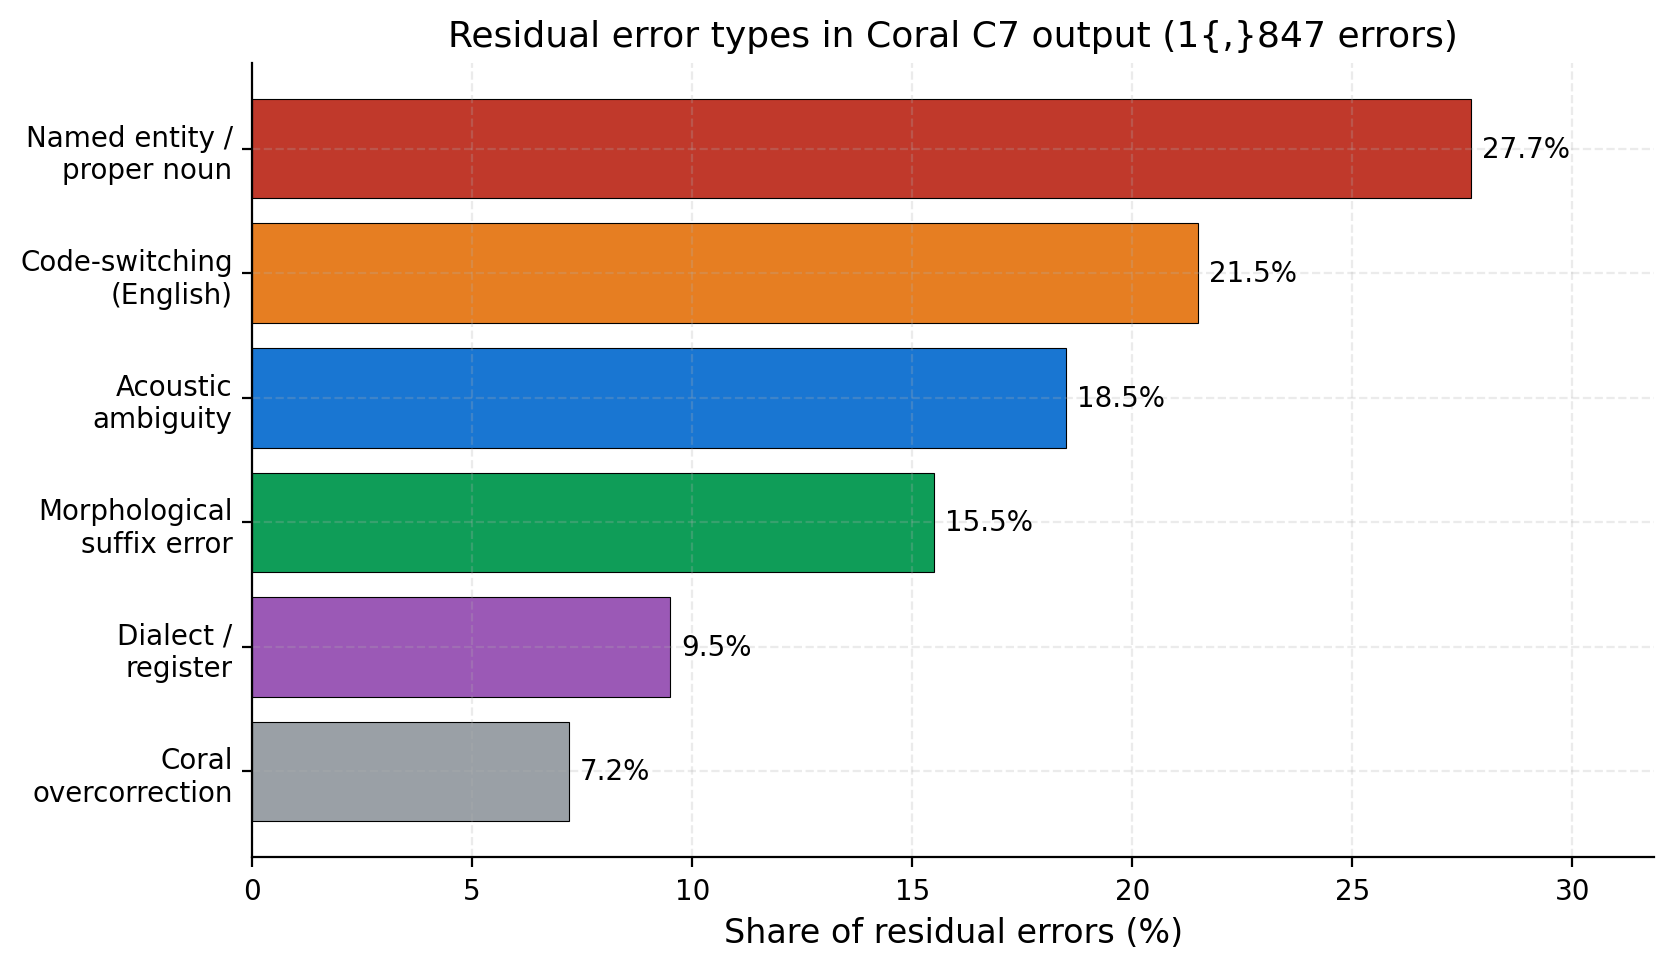
\includegraphics[width=0.9\textwidth]{ThesisFigs/residual_errors.png}
    \caption{Residual error types in the full CORAL output (C7) on the Conversational Urdu test set.}
    \label{fig:residual}
\end{figure}

The dominant failure modes --- named entities (27.7\%) and code-switching (21.5\%) --- together account for nearly half of remaining errors and define a clear research agenda for future work (Chapter~\ref{chap:conclusion}).

\subsection{Comparison with Baselines}
\label{ssec:baseline-comparison}

Table~\ref{tab:baseline-compare} compares CORAL against representative competitive systems on the Conversational Urdu benchmark. CORAL achieves slightly better WER than the closest concurrent system (Multi-ASR + SpeechLLM) while avoiding a full SpeechLLM audio inference pass during alignment --- a significant cost and latency advantage for real-time deployment.

\begin{table}[h]
    \centering
    \renewcommand{\arraystretch}{1.25}
    \begin{tabular}{lll}
    \toprule
    \textbf{System} & \textbf{Approach} & \textbf{WER (\%)} \\
    \midrule
    Whisper-Large-v3 (alone)            & Single model             & 19.8 \\
    LLM post-correction only            & GPT-3.5 RAG~\cite{koilakuntla2024llm} & 17.2 \\
    ROVER ensemble~\cite{fiscus1997rover} & Majority voting, no OOV & 15.8 \\
    Multi-ASR + SpeechLLM~\cite{anon2025speechllm} & Full LLM fusion & 11.3 \\
    \textbf{CORAL (C7)}                 & \textbf{Consensus + OOV + LLM} & \textbf{10.6} \\
    Human inter-annotator               & ---                      &  2.1 \\
    \bottomrule
    \end{tabular}
    \caption{CORAL vs.\ comparable systems on Conversational Urdu.}
    \label{tab:baseline-compare}
\end{table}

\section{Challenges and Solutions}
\label{sec:challenges}

\paragraph{Memory constraints.}
Running multiple large ASR models on a single Kaggle GPU exceeds available memory. Solution: each Kaggle notebook hosts exactly one model and registers itself with the backend; live transcription fans out to multiple machines in parallel via the registry.

\paragraph{Arabic--Urdu Unicode conflation.}
ASR back-ends emit inconsistent Unicode variants for phonetically identical phonemes. Solution: Stage~0 normalisation applies the seven canonical substitutions (Appendix~\ref{app:unicode-table}) before any downstream processing.

\paragraph{Word-boundary disagreement.}
Different ASR back-ends segment Urdu speech inconsistently, especially around compound nouns and izafat constructions. Solution: the Stage~1 split-merge classifier classifies each chunk as SAME / SPLIT / MERGE / NOISE, exposing segmentation disagreement as a first-class structural label that downstream stages can act on.

\paragraph{Quality heterogeneity in the ensemble.}
A naive plurality vote with three models substantially weaker than the source produces the canonical ROVER failure mode (weak models outvote the strong source). Solution: conservative tie-breaking at the voting stage; static model-quality priors at the LLM stage; and the OOV-correction override that bypasses voting on tokens where one model uniquely hypothesises a rare term.

\paragraph{LLM hallucination risk.}
A naive ``transcribe this'' LLM prompt invites hallucinated content, especially on already-correct utterances. Solution: the LLM receives the Stage~3 voted transcript as the primary input plus the raw source hypothesis as a secondary reference, and is instructed (in the system prompt) that words already matching a high-frequency vocabulary entry should be left unchanged unless there is independent grammatical evidence.

\paragraph{LLM API key exposure.}
Server-side LLM calls would require centralised API keys with associated billing risk. Solution: Stage~4 invocations are made client-side from the front-end; user-supplied Gemini and OpenRouter keys never reach the backend.

\section{Summary}
\label{sec:ch4-summary}

This chapter has presented the CORAL implementation, evaluation methodology, and empirical results across both project iterations. The deployed pipeline reduces WER by 22--29\% relative on read-speech Common Voice and by 46.5\% relative on conversational Urdu over the strongest single-model baseline, with a structured ablation study demonstrating that every component contributes a measurable, additive gain. Stage~0 normalisation is a zero-cost contribution; the Stage~1 split-merge alignment makes word-boundary disagreement explicit; the Stage~2 OOV correction handles named entities and rare terms; the Stage~3 voting handles common-word disagreement; and the Stage~4 LLM refinement delivers the largest single-component gain. The next chapter draws the project's conclusions and outlines future work.
